%SourceDoc ws-skript.tex
%
% c01-wahrscheinlichkeit.tex -- 1. Kapitel, Wahrscheinlichkeitsbegriff
%
% (c) 2006 Prof. Dr. Andreas Mueller, HSR
% $Id: c01-wahrscheinlichkeit.tex,v 1.24 2008/09/15 23:49:57 afm Exp $
%
\rhead{Ereignisse und Wahrscheinlichkeit}
\chapter{Ereignisse und ihre Wahrscheinlichkeit\label{chapter-ereignisse-und-wahrscheinlichkeit}}
Es ist unm"oglich den Ausgang eines Sportwettkampfes vorauszusagen.
Trotzdem trauen sich viele Leute zu, auf Grund ihrer Kenntnisse "uber den
Trainingsstand der Sportler ihrer fr"uheren Leistungen, Prognosen abzugeben.
Sie sind sich dabei oft so sicher, dass sie bereit sind, Geld auf ihren Tipp
zu wetten.
Eine solche Prognose ist nicht immer gleich schwierig. Wenn an der
Fussball WM der Favorit Brasilien gegen Ghana antritt,
rechnet wohl niemand ernsthaft mit einem Sieg Ghanas. Die Leute w"urden
sagen, es sei unwahrscheinlich, dass das Ereignis ``Ghana gewinnt'' eintreffen
w"urde. Anders sieht es aus, wenn die Schweiz auf die Ukraine trifft.
Die Prognosen "uber den Ausgang dieses Matches waren auch abseits
manchmal etwas chauvinistischer Hoffnungen mindestens uneinheitlich.

Wie auch immer, die einzige M"oglichkeit herauszufinden, welche Mannschaft
st"arker ist, besteht darin, das Spiel tats"achlich durchzuf"uhren.
Vorher w"urden wir einen Sieg der Schweizer Nati bestenfalls als
wahrscheinlich oder eher unwahrscheinlich einstufen.
Welche der beiden M"oglichkeiten tats"achlich eintritt, l"asst sich
erst nach dem Spiel sagen.

Wir haben also ein Ereignis, n"amlich einen Sieg der Schweizer Nati,
und sind mindestens gef"uhlsm"assig in der Lage, dem Eintreten dieses
Ereignis eine Wahrscheinlichkeit zuzuordnen.
Eine Sicherheit haben wir aber nicht. 
Dazu m"ussen wir das Experiment durchf"uhren, und sehen dann,
welches Ereignis, Sieg oder Niederlage eingetreten ist.

Die Wahrscheinlichkeitsrechnung will solchen Aussagen einen pr"azisen
mathematischen Sinn geben. Daher brauchen wir zun"achst Definitionen
f"ur die Begriffe ``Ereignis'' und ``Wahrscheinlichkeit''.  Mit geeigneten
Rechengesetzen sollte die Wahrscheinlichkeit berechnet werden k"onnen,
und wir sollten eine rationale Grundlage f"ur Sportwetten finden k"onnen.

\section{Ereignisse\label{section-begriffe}}
\index{Ereignis}
Zun"achst brauchen wir mathematisch scharfe Begriffe f"ur die Begebenheiten
in der realen Welt, welche wir mit der Wahrscheinlichkeitsrechnung behandeln
wollen. Wenn die Wahrscheinlichkeitsrechnung in die Lage versetzen soll,
darauf wetten zu k"onnen, das etwas passiert oder eben nicht, dann braucht
sie offensichtlich eine Definition des Begriffes {\bf Ereignis}.
\marginpar{\tiny Begriff des Ereignisses}
Ereignisse treten ein, oder eben nicht.
Als solche kann man Ereignisse oft mit einfachen S"atzen festhalten:
\begin{enumerate}
\item Der Blitz hat in den Baum eingeschlagen.
\item Der W"urfel zeigt eine Sechs.
\item Das Flugzeug ist "uber die Piste hinausgerast.
\item Hans hatte einen Sechser im Lotto.
\end{enumerate}
In diesen S"atzen steckt implizit die Beschreibung eines Experimentes oder
Vorgangs, die Feststellung h"alt nur den Ausgang fest:
\begin{enumerate}
\item Beim letzten Gewitter gabe es nat"urlich eine grosse
Zahl von Blitzen.
Am Ende des Gewitters stand fest, dass einer der Blitze den Baum
getroffen hat.
\item Der W"urfel kann eine komplizierte Bahn beschreiben, und wenn
er nach dem W"urfeln auf dem Tisch liegt, kann er in verschiedene
Richtungen orientiert sein. Entscheidend ist jedoch nur das Ergebnis,
welche Zahl oben liegt.
\item Die meisten Flugzeuge starten oder landen erfolgreich, d.~h.~sie
heben ab oder kommen rechtzeitig zum Stillstand. Hin und wieder
endet ein Start- oder Landeversuch jedoch mit einem anderen Ausgang,
in diesem Fall eben damit, dass das Flugzeugt "uber die Piste
hinausgerast ist.
\item Hans hat einen Lottozettel ausgef"ullt, und die Lottogesellschaft
hat Lottozahlen gezogen. Danach wurde der Lottozettel mit den Zufallszahlen
verglichen. Der Ausgang dieses Experiments zeigt sechs "Ubereinstimmungen.
\end{enumerate}
Dieser Begriff des Ereignisses ist offenbar sehr weit gespannt.
Um ihn in mathematische brauchbare Form zu bringen,
muss man sich zun"achst "uberlegen, welche Eigenschaften Ereignisse haben
sollen.

Bevor wir eine mathematische Beschreibung von Ereignissen versuchen,
wollen wir deshalb an einem popul"aren Beispiel die relevanten Ereignisse
formulieren.

\subsection{AIDS-Test\label{aids-test-intro}}
Wenn sich jemand im Bezug auf AIDS riskant verhalten hat, dann ist
eine seiner Sorgen, dass der AIDS-Test nicht sofort das richtige
Resultat anzeigt. Und selbst wenn er die notwendige Frist abgewartet
hat, hat der Test eine geringe Fehlerrate.
Es k"onnen also verschiedene Ereignisse eintreten. Meistens wird ein
positiver AIDS-Test richtig anzeigen, dass eine Person HIV hat. Manchmal
wird der Test jedoch positiv sein, obwohl die Person gesund ist. Und manchmal
wird der Test zwar ein positives Resultat zeigen, aber die Person ist
an HIV erkrankt. Gl"uck haben diejenigen, bei denen der Test nicht
anspricht, und die auch tats"achlich gesund sind.


\subsection{Euromillions}
\index{Euromillions}
\begin{figure}
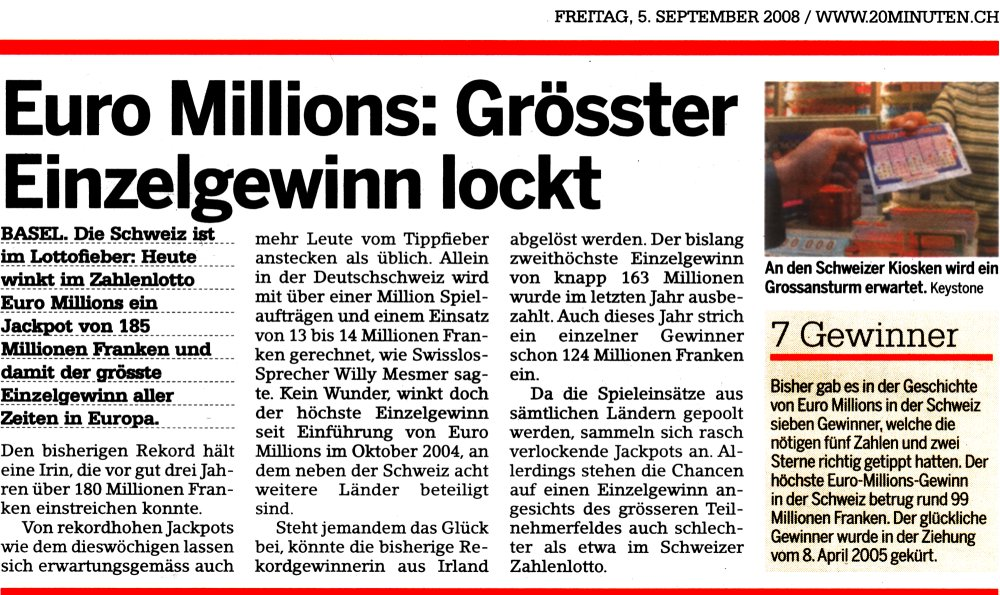
\includegraphics[width=\hsize]{graphics/euromillions}
\caption{Besondere Gewinnchance in Euromillions}
\end{figure}
\begin{figure}
\begin{center}
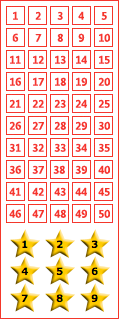
\includegraphics[height=8cm]{graphics/euromillionsschein}
\end{center}
\caption{Teilnahmeschein f"ur Euromillions\label{euromillionsschein}}
\end{figure}
Am 5.~September 2008 schrieb die Gratiszeitung ``20 Minuten'', dass die
bevorstehende Ziehung der Lotterie Euromillions besondere Gewinnschancen 
erm"ogliche, weil der Jackpot ungew"ohnlich gross sei. Welche Ereignisse
sind in diesem Spiel relevant?

Auf der Euromillions-Website findet man die Erkl"arung, wie das Spiel abl"auft.
Der Spieler kreuzt auf dem Teilnahmeschein (Abbildung~\ref{euromillionsschein})
f"unf Zahlen und zwei Sterne an. Dann erfolgt die Ziehung, Euromillions ermittelt
5 Gewinnzahlen aus dem Bereich 1--50 und 2 Gewinnsterne im Bereich 1--9.
Jetzt werden die "Ubereinstimmungen zwischen dem Tipp des Teilnehmers und den
Gewinnzahlen gez"ahlt. Je besser die "Ubereinstimmung desto gr"osser der Gewinn.

\begin{table}
\begin{center}
\begin{tabular}{|c|c|c|c|}
\hline
Gewinnrang&richtige Zahlen&richtige Sterne&Anteil Gewinnsumme\\
\hline
1&5&2&32.0\%\\
2&5&1&7.4\%\\
3&5&0&2.1\%\\
4&4&2&1.5\%\\
5&4&1&1.0\%\\
6&4&0&0.7\%\\
7&3&2&1.0\%\\
8&3&1&5.1\%\\
9&2&2&4.4\%\\
10&2&0&4.7\%\\
11&1&2&10.1\%\\
12&2&1&24.0\%\\
\hline
\end{tabular}
\end{center}
\caption{Gewinnr"ange bei Euromillions\label{gewinnraenge}}
\end{table}

Die Tabelle \ref{gewinnraenge} zeigt, wie der Gewinn verteilt wird.
Offenbar spielen dabei sogenannte Gewinnr"ange eine besondere Rolle.
Bei jedem Tippzettel wird festgestellt, in welchen Gewinnrang er
geh"ort.

Ausser den Gewinnr"angen k"onnen auch andere Ereignisse eintreten,
die jedoch f"ur die Auszahlung nicht unbedingt von Bedeutung sind,
oder aus denen sich der Gewinn noch nicht ableiten l"asst:
\begin{itemize}
\item {\it Heiris Euromillions Teilnahmeschein f"allt in Gewinnrang 10.} Offenbar
teilt sich Heiri 4.7\% der Gewinnsumme mit den anderen Teilnehmern, die
dasselbe Ergebnis erziehlt haben.
\item {\it Hanna hatte f"unf richtige Zahlen.} Diese Information reicht noch
nicht, um den Gewinn festzulegen. Hannas Teilnahmeschein f"allt in
Gewinnrang 1 oder 2 oder 3.
\item {\it Hermine hatte keinen einzigen Stern richtig.} Hermine k"onnte
etwas gewonnen haben, n"amlich wenn sie 5, 4 oder 2 richtige Zahlen
gehabt hat (R"ange 3, 6 bzw.~10). Oder sie k"onnte mit 3, 1 oder 0
richtigen Zahlen nichts gewonnen haben.
\item {\it Hermann hatte richtige Zahlen und Sterne.} Hermann hatte
als 1, 2, 3, 4 oder 5 richtige Zahlen {\bf und}
1 oder 2 richtige
Sterne.
\item {\it Es trifft nicht zu, dass Hilary einen richtigen Stern hat.}
\item {\it Holger hat auf 47 gesetzt.}
Dieses Ereignis nimmt auf die Ziehung "uberhaupt keinen Bezug,
trotzdem beschreibt es einen m"oglichen Ausgang des Experimentes.
\end{itemize}
Wir stellen fest, dass Ereignisse mit {\bf und} (beide Ereignisse sind
eingetreten) und {\bf oder} (eines der Ereignisse ist
eingetreten) verkn"upft werden k"onnen. Ausserdem k"onnen 
Ereignisse negiert werden.

\subsection{Eigenschaften von Ereignissen}
Man kann aus Ereignissen neue Ereignisse bilden:
\begin{enumerate}
\item Dass zwei Ereignisse gleichzeitig eintreten ist ebenfalls ein
Ereignis.
\item Dass von zwei Ereignissen eines eintreten kann, ist ebenfalls
ein Ereignis.
\item Dass ein Ereignis nicht eintritt, ist ebenfalls ein Ereignis.
\end{enumerate}
Ausserdem kann es sein, dass ein Ereignis nur eintreten kann, wenn ein
anderes Ereignis bereits eingetreten ist.

Ereignisse brauchen nicht etwas unteilbares
zu sein, denn wenn man ``genauer hinschaut'',
kann ein Ereignis aus einer
grossen Zahl von Einzelereignissen bestehen, die das beobachtete Resultat
herbeif"uhren. Wenn man einen Stapel Karten mischt, sich aber nur daf"ur
interessiert, welche Farbe die oberste Karte hat, ist dies offenbar mit einer
sehr grossen Zahl von m"oglichen Anordnungen der "ubrigen Karten m"oglich.
Umgekehrt ist es sehr gut m"oglich, dass es keine praktische M"oglichkeit
gibt, ``genauer hinzuschauen'', in diesem Fall l"asst sich ein Ereignis
nicht weiter zerteilen, man k"onnte von einem Elementarereignis\marginpar{\tiny Elementarereignis} sprechen.
\index{Elementarereignis}

Manchmal interessiert bei einem Versuchsverlauf nur ein einziges Attribut,
zum Beispiel wird sich niemand f"ur alle Einzelheiten eines Versuchs
interessieren die zu einem bestimmten Messwert gef"uhrt haben. Die Messung 
gruppiert also Ereignisse, die zu einem bestimmten Messwert f"uhren, zu
einem gr"osseren Ereignis.

\subsection{Mathematische Modellierung von Ereignissen}
Die Mengenlehre bildet den nat"urlichen Rahmen f"ur die Operationen,
die wir f"ur Ereignisse ben"otigen.
Die Elementarereignisse sind gute Kandidaten daf"ur, eine geeignete
Grundmenge abzugeben. Ereignisse
\marginpar{\tiny Ereignisse als Mengen}
k"onnen mehrere Elementarereignisse umfassen, die alle zum gleichen
``Ausgang'' f"uhren.
Sie sind also Mengen von Elementarereignissen. Um die Begriff festzulegen
verwenden wir f"ur die Menge der Elementarereignisse den Buchstaben $\Omega$.
Elementarereignisse sind also Elemente $\omega\in\Omega$, Ereignisse sind
Teilmengen $A\subset\Omega$.

Beispiel: Der Wurf eines W"urfels ist ein Zufallsexperiment, von dem im
Moment nur die oben liegende Zahl als Ausgang interessiert, nicht die 
komplizierte Flugbahn des W"urfels, bis er endlich ruhig liegt.
Elementarereignisse sind in dieser Sicht die Zahlen
$\Omega = \{1, 2, 3, 4, 5, 6\}$.
Ereignisse sind Teilmengen von $\Omega$. Das Ereignis
``es wurde eine gerade Augenzahl geworfen'' ist die Menge $\{2, 4, 6\}$.

Bei\marginpar{\tiny Eintreten von Ereignissen} einem Zufallsexperiment
wird irgend eines der m"oglichen
Elementarereignisse in $\Omega$ realisiert, nennen wir es $\omega$.
Das Ereignis $A\subset\Omega$
tritt ein, wenn $\omega\in A$ ist. Im W"urfelbeispiel tritt das Ereignis
``es wurde eine ganze Zahl geworfen'' also zum Beispiel ein, wenn eine
2, 4 oder 6 gew"urfelt wird.

Zwei Ereignisse $A\subset\Omega$ und $B\subset\Omega$ treten bei einem
Versuch gleichzeitig\marginpar{\tiny Gleichzeitiges Eintreten von Ereignissen}
ein, wenn das realisierte Elementarereignis
$\omega$ sowohl in $A$ als auch in $B$ liegt, also $\omega\in A\cap B$.
Wenn die Ereignisse $A=\{\hbox{gerade Zahl}\}$ und
$B=\{\hbox{durch $3$ teilbare Zahl}\}$ gleichzeitig eintreten, dann
gilt
\[
A\cap B = \{2, 4, 6\} \cap \{3, 6\} = \{6\},
\]
es wurde also eine $6$ gew"urfelt.

Zwei Ereignisse sind speziell.
Die Menge $\Omega\subset\Omega$ hat die Eigenschaft, dass jeder denkbare
Versuchsausgang per Definition in $\Omega$ liegt, das Ereignis $\Omega$
tritt also immer ein. $\Omega$ heisst daher auch das\marginpar{\tiny sicheres Ereignis} sichere Ereignis.
\index{Ereignis!sicheres}
Die leere Menge $\emptyset\subset\Omega$ hat genau die gegenteilige
Eigenschaft: was auch immer geschieht, was auch immer f"ur ein 
Elementarereignis $\omega$ realisiert wird, in $\emptyset$ kann es
nicht drin sein, also wird $\emptyset$ nie eintreten. $\emptyset$
heisst daher auch das unm"ogliche
Ereignis\marginpar{\tiny unm"ogliches Ereignis}.
\index{Ereignis!unm\"ogliches}

\begin{table}
\begin{center}
\begin{tabular}{|l|c|}
\hline
Begriff&Modell\\
\hline
Elementarereignis&$\omega$\\
alle Elementarereignisse&$\Omega$\\
Ereignis&$A\subset\Omega$\\
sicheres Ereignis&$\Omega$\\
unm"ogliches Ereignis&$\emptyset$\\
$A$ und $B$&$A\cap B$\\
$A$ oder $B$&$A\cup B$\\
$A$ hat $B$ zur Folge, $A\Rightarrow B$&$A\subset B$\\
nicht $A$&$\Omega\setminus A$\\
\hline
\end{tabular}
\end{center}
\caption{Begriffe der Wahrscheinlichkeitstheorie und ihre mathematischen
Modellierung\label{begriffe-zusammenfassung}}
\end{table}

Auch andere Mengenoperationen und Relationen haben Entsprechungen
in der Begriffswelt der Ereignisse. Sind $A$ und $B$ zwei Ereignisse
mit $A\subset B\subset\Omega$, dann tritt offensichtlich $B$ auf
jeden Fall dann ein, wenn $A$ eingetreten ist. Wird n"amlich $\omega\in A$
realisiert, dann ist auch $\omega\in B$. Man kann auch sagen, $A$ impliziert
$B$, oder $A$ hat $B$ zur Folge, $A\Rightarrow B$.

Die Vereinigungsmenge\marginpar{\tiny Vereinigung von Ereignissen}
zweier Ereignisse $A$ und $B$ besteht aus jenen
Elementarereignissen, die in $A$ oder in $B$ liegen. $A\cup B$ tritt
also ein, wenn das realisierte Elementarereignis $\omega\in A$
oder $\omega\in B$ liegt.

Das Ereignis\marginpar{\tiny negiertes Ereignis}
``$A$ tritt nicht ein'', oder $\lnot A$, besteht aus
jenen Elementarereignissen, die nicht in $A$ liegen,
also $\lnot A=\Omega\setminus A$.

Die eben entwickelten Begriffe sind in der Tabelle
\ref{begriffe-zusammenfassung} zusammengefasst.
\index{Ereignisalgebra}

\subsection{Produkte}
\begin{figure}
\begin{center}
\begin{tabular}{|c|c|c|c|c|c|}
\hline
(1,1)&(1,2)&(1,3)&(1,4)&(1,5)&(1,6)\\
\hline
(2,1)&(2,2)&(2,3)&(2,4)&(2,5)&(2,6)\\
\hline
(3,1)&(3,2)&(3,3)&(3,4)&(3,5)&(3,6)\\
\hline
(4,1)&(4,2)&(4,3)&(4,4)&(4,5)&(4,6)\\
\hline
(5,1)&(5,2)&(5,3)&(5,4)&(5,5)&(5,6)\\
\hline
(6,1)&(6,2)&(6,3)&(6,4)&(6,5)&(6,6)\\
\hline
\end{tabular}
\end{center}
\caption{Elementarereignisse f"ur das W"urfeln mit zwei unterscheidbaren
W"urfeln\label{ereignisse-zwei-wuerfel}}
\end{figure}
Wir stellen uns vor, dass ein roter und ein blauer W"urfel geworfen werden.
Die von den beiden W"urfeln gezeigten Augenzahlen sind verschiedene
Versuchsausg"ange, sozusagen ``rote'' und ``blaue'' Zahlen. Das Resultat
eines Wurfes ist also ein Paar bestehend aus einer ``roten'' und
einer ``blauen'' Augenzahl. Die Menge aller m"oglichen Ausg"ange
ist also 
\[
\Omega = \Omega_{\text{rot}}\times\Omega_{\text{blau}},
\]
das kartesische Produkt der Mengen $\Omega_{\text{rot}}$ und
$\Omega_{\text{blau}}$ (siehe auch Abbildung \ref{ereignisse-zwei-wuerfel}).

In $\Omega$ lassen sich bereits bedeutend spannendere Ereignisse
beschreiben:
\begin{eqnarray*}
A_1&=&\{\text{mindestens eine ungerade Zahl}\}\\
   &=&\{(x,y)\in\Omega\;|\;x \equiv 1\mod 2 \vee y\equiv 1\mod 2\}\\
A_2&=&\{\text{beide Augenzahlen sind gerade}\}\\
   &=&\{(x,y)\in\Omega\;|\;2|x \wedge 2|y\}\\
X_i&=&\{(i,y)\in\Omega\}\\
Y_i&=&\{(x,i)\in\Omega\}\\
S_s&=&\{(x,y)\in\Omega\;|\; x + y = s\}\\
D_d&=&\{(x,y)\in\Omega\;|\; |x - y| = d\}\\
\end{eqnarray*}
Und damit lassen sich auch etwas spannendere Rechnungen durchf"uhren. Zum
Beispiel:
\begin{eqnarray*}
A_1&=&\Omega \setminus A_2 = \bar A_2\\
A_1\cap A_2&=&\emptyset\\
A_1&=&X_1\cup X_3 \cup X_5\cup Y_1\cup Y_3\cup Y_5\\
X_4\cap Y_3&=&\{(4,3)\}\\
X_5\cap S_7&=&\{(5,2)\}\\
X_5\cap D_1&=&\{(5,4), (5,6)\}\\
\end{eqnarray*}
%Beweise: "Ubungsaufgaben.

%Allgemein lassen sich also zwei Ereignisalgebren $(\Omega_1,{\cal A}_1)$
%\marginpar{\tiny Produkt von Ereignisalgebren}
%und $(\Omega_2,{\cal A}_2)$ zu einer neuen Ereignisalgebra
%kombinieren, indem man deren Kreuzprodukt 
%$(\Omega, {\cal A})=(\Omega_1,{\cal A}_1)\times(\Omega_2,{\cal A}_2)$
%bildet. Die Menge der Elementarereignisse ist $\Omega = \Omega_1\times\Omega_2$,
%aber die Menge der Ereignisse $\cal A$ ist nicht so leicht anzugeben.
%Ausser aus den Produkte von je einem Ereignis aus ${\cal A}_1$ und
%${\cal A}_2$ sind auch alle Durchschnitte, Vereinigungen und Komplemente
%von solchen Produkten in $\cal A$.

\subsection{*Abbildungen}
Wir betrachten wieder das Beispiel $(\Omega,\cal A)$
zweier unterscheidbarer W"urfel. Daneben
interessieren wir uns daf"ur, dass eine bestimmte Summe von Augenzahlen
gew"urfelt wird. Die m"oglichen Ausg"ange (Elementarereignisse)
f"ur diese zweite Art von
Experiment ist die Menge der ganzen Zahlen von 1 bis 12,
$\Omega'=\{n\in\mathbb N\;|\;1 \le n \le 12\;\}$, und die
Menge der Ereignisse ist die Menge aller Teilmengen
${\cal A}'={\cal P}(\Omega')$.

Offensichtlich gibt es eine Abbildung $s\colon \Omega\to\Omega'$, die 
die Summe der Augenzahlen ausrechnet:
\[
s\colon\Omega\to\Omega':(x,y)\mapsto x+y
\]
Das Eintreten eines bestimmten Elementarereignisses $a \in\Omega'$
bedeutet jetzt, dass in $\Omega$ das Ereignis $S_a$ eingetreten
ist. 

\subsection{Formale Definition}
Im Allgemeinen wird es gen"ugen, Mengen von Ereignissen
$A\subset\Omega$ zu betrachten, f"ur die sich alle obigen
Operationen durchf"uhren lassen. Die Menge aller Teilmengen von
$\Omega$, die Potenzmenge ${\cal P}(\Omega)$ erf"ullt diese Bedingung,
ist aber sehr gross und hat sehr wenig n"utzliche Struktur, die
f"ur den Aufbau des Begriffs der Wahrscheinlichkeit im n"achsten
Abschnitt ben"otigt wird.  Damit gelangen wir zu folgender Definition
einer Ereignis-Algebra:

\begin{definition}
\label{def-ereignisalgebra}
Eine Ereignisalgebra $(\Omega,{\cal A})$ ist
eine Menge $\Omega$ mit einer Menge ${\cal A }\subset{\cal P}(\Omega)$
von Teilmengen von $\Omega$, die folgende Bedingungen erf"ullen:
\begin{enumerate}
\item Vereinigungen von Elementen von ${\cal A}$ sind ebenfalls in ${\cal A}$,
also
\[
A,B\in {\cal A}\Rightarrow A\cup B\in{\cal A}
\]
\item Differenzen von Elementen von ${\cal A}$ sind in ${\cal A}$, also
\[
A,B\in {\cal A}\Rightarrow A\setminus B\in{\cal A}
\]
\item $\Omega\in{\cal A}$, d.h. es gibt das sichere Ereignis.
\end{enumerate}
\end{definition}

Sind nur die Bedingungen 1 und 2 erf"ullt, spricht man auch von einem
Mengen-Ring. Eine Ereignisalgebra heisst manchmal auch ein Mengen-K"orper.

Aus den Axiomen f"ur die Ereignisalgebra lassen sich sofort erst
Schlussfolgerungen ziehen:
\begin{enumerate}
\item Es gibt auch das unm"ogliche Ereignis: $\emptyset = \Omega\setminus\Omega\in{\cal A}$.
\item Das Komplement eines Ereignisses ist ebenfalls ein Ereignis: $\bar A=\Omega\setminus A\in{\cal A}$.
\item Der Durchschnitt zweier Ereignisse ist ebenfalls ein Ereignis: $A\cap B = 
(A\cup B) \setminus ((A\setminus B) \cup (B\setminus A))\in{\cal A}$.
\end{enumerate}

\section{Beispiele\label{section-beispiele}}
\subsection{Dominosteine}
Die Menge aller m"oglichen Dominosteine wurde bereits fr"uher untersucht.
Jetzt m"ochten wir darin einzelne Ereignisse auszeichnen. Wir beschreiben
einen einzelnen Dominostein als ein paar $(x,y)$, wobei $x\ge y$ sein soll.
Beispiele von Ereignissen:
\begin{align*}
S_k&=\{ \text{Die Augensumme ist $k$}\}\\
S_5&=\{ (5,0), (4,1), (3,2) \}\\
S_4&=\{ (4,0), (3,1), (2,2) \}\\
R&=\{\text{die Augenzahlen sind positiv haben keinen gemeinsamen Teiler $>1$}\}\\
 &=\{ (6,5), (6,1), (5,4), (5,3), (5,2), (5,1), (4,3), (4,1), (3,2), (3,1), (2,1), (1,1) \}
\\
P&=\{\text{beide Augenzahlen sind Primzahlen}\}\\
 &=\{(5,5), (5,3), (5,2), (3,3), (3,2), (2,2) \}\\
\end{align*}

\subsection{W"urfeln mit zwei W"urfeln}
Bei einem W"urfelspiel wirft man jeweils zwei W"urfel. Zeigen beide W"urfel
die gleiche Zahl, man nennt dies einen Pasch, darf man genau einmal w"urfeln.
Die Elementarereignisse sind also entweder einfach Paare, also von
der Form $(x,y)$, mit $x\ne y$, oder ein Pasch gefolgt von irgend einem
W"urfelresultat, wir schreiben dies $(P_k, (x,y))$, also ein $k$-er-Pasch
gefolgt von einem Paar $(x,y)$, wobei diesmal keine Einschr"ankungen f"ur
$x$ und $y$ gelten.
Damit kann man jetzt alle m"oglichen Elementarereignisse auflisten
\begin{align*}
\Omega=\{
&\phantom{(6,6),} (6,5), (6,4), (6,3), (6,2), (6,1)\\
&(5,6), \phantom{(5,5),} (5,4), (5,3), (5,2), (5,1)\\
&(4,6), (4,5), \phantom{(4,4),} (4,3), (4,2), (4,1)\\
&(3,6), (3,5), (3,4), \phantom{(3,3),} (3,2), (3,1)\\
&(2,6), (2,5), (2,4), (2,3), \phantom{(2,2),} (2,1)\\
&(1,6), (1,5), (1,4), (1,3), (1,2), \phantom{(1,1)}
\}
\\
&\cup
\{(P_6,(x,y))\}
\cup
\{(P_5,(x,y))\}
\cup
\{(P_4,(x,y))\}
\\
&\cup
\{(P_3,(x,y))\}
\cup
\{(P_2,(x,y))\}
\cup
\{(P_1,(x,y))\}
\end{align*}
Man sieht daraus zum Beispiel, dass es $30 + 6\cdot 36=246$
Elementarereignisse gibt. Darin enthalten sind die Ereignisse
\begin{align*}
P&=\{\text{Pasch im ersten Wurf}\}\\
&=
\{(P_6,(x,y))\}
\cup
\{(P_5,(x,y))\}
\cup
\{(P_4,(x,y))\}
\\
&\qquad \cup
\{(P_3,(x,y))\}
\cup
\{(P_2,(x,y))\}
\cup
\{(P_1,(x,y))\}
\\
P_k&=\{\text{$k$-er Pasch im ersten Wurf}\}\\
   &=\{(P_k,(x,y))\}
\\
Q&=\{\text{totale Augensumme $\ge 10$}\}\\
&=\{\phantom{(6,6),} (6,5), (6,4), \\
&\phantom{\;=\{}(5,6), \phantom{(5,5),} \\
&\phantom{\;=\{}(4,6)
\}
\\
&\qquad\cup
\{(P_6,(x,y))\}
\cup
\{(P_5,(x,y))\}
\cup
\{(P_4,(x,y))\,|\, x+y \ge 2\}
\\
&\qquad\cup
\{(P_3,(x,y))\,|\, x+y \ge 4\}
\cup
\{(P_2,(x,y))\,|\, x+y \ge 6\}
\\
&\qquad
\cup
\{(P_1,(x,y))\,|\, x+y \ge 8\}
\end{align*}

\subsection{AIDS-Test}
Wir mathematisieren das Beispiel des AIDS-Tests.
Die Diskussion in \ref{aids-test-intro} f"uhrt uns vor Augen,
dass wir hier mit zwei verschiedenen Ereignissen zu tun haben. 
Das Experiment besteht offenbar darin, dass wir jemanden Untersuchen,
die Menge Elementarereignisse ist also die Menge aller betrachteten Personen.
Darin unterschieden wir:
\begin{align*}
H&=\{\text{Person hat HIV}\}\\
T&=\{\text{Person hat positiven AIDS-Test}\}
\end{align*}
Es ist klar, dass $H\ne T$. Es gibt Personen, die zwar HIV haben, bei
denen der Test dies aber noch nicht zeigen kann, $H\setminus T\ne \emptyset$.
Andererseits gibt es falsche positive Testresultate,
$T\setminus H\ne\emptyset$. 

%\subsection{Zwei ununterscheidbare W"urfel}
%Wir stellen uns zwei vollkommen ununterscheidbare W"urfel vor. Genau
%genommen ist dies in der makroskopischen Welt nicht m"oglich, es l"asst
%sich da immer ein Unterscheidungsmerkmal finden. In der mikroskopischen
%Welt hingegen gibt es durchaus ununterscheidbare Teilchen, die in
%verschiedenen Zust"anden sein k"onnen, wir k"onnten diese als
%ununterscheidbare W"urfel ansehen.
%
%Wenn wir uns wieder nur f"ur den Ausgang des W"urfelns mit den zwei
%ununterscheidbaren W"urfeln interessieren, d"urfen wir das Resultat
%$(x,y)$ nicht mehr von $(y,x)$ unterscheiden. Bei unterscheidbaren
%W"urfeln war dies m"oglich, die erste Position war f"ur die
%Augenzahl des roten W"urfels reserviert. Daher ist die Menge der
%m"oglichen Ausg"ange nun nur noch
%$\{(x,y)|1\le x,y\le 6\wedge x\le y\}$.

%\subsection{Ein komplexeres Beispiel: die Fussball WM 2006}
%Betrachten wir alle m"oglichen Spiele an einer Fussball WM.
%Offensichtlich ist dies eine ungeheuer grosse Menge. An Stammtischen
%rund um die Welt wurden alle m"oglichen F"alle diskutiert, wie
%Spiele anders h"atten ausgehen k"onnen. Und selbst alle dies Theorien
%machen nur einen kleinen Teil aller m"ogliche Spiele aus.
%Wir bezeichnen diese Menge mit $\Sigma$.
%Jedes Element $x\in\Sigma$ ist also ein denkbares
%Spiel. "Uber jedes Spiel gibt es sehr viel Information, zum Beispiel
%hat jedes Spiel zwei Teilnehmermannschaften, selbst dann, wenn diese
%dem Match fernbleiben, wie im Spiel Schweiz -- Togo beinahe geschehen.
%
%Bei der tats"achlichen Durchf"uhrung der WM werden nur einige ganz wenige
%dieser Spiele tats"achlich real. W"ahrend den Fussballfans nat"urlich unz"ahlige
%Einzelheiten eines Spiels wichtig sind, z"ahlt am Schluss nur noch die Zahl
%der Tore, die die beiden Mannschaften erzielt haben. An der Fussball WM 2006
%fand zum Beispiel ein Spiel Schweiz gegen S"udkorea statt. Auch dieses Spiel
%h"atte auf viele Arten ausgehen k"onnen, die Menge
%$$\{\text{Die Schweiz spielt gegen S"udkorea}\}\subset\Sigma$$
%ist also eine Teilmenge aller m"oglichen Spiele. Wenn man sich heute noch
%an den Ausgang des Spieles erinnert, kennt man nur noch die Menge
%$$\sigma=\{\text{Die Schweiz besiegt S"udkorea 2 : 0}\}\subset\Sigma.$$
%Aber selbstverst"andlich ist auch dies eine sehr grosse Menge,
%die Stadionbesucher am 23.~Juni 2006 in Hannover
%haben ein Realisation $x\in\sigma$ gesehen.
%
%Die WM selbst besteht aus einer Folge von Spielen. Nach einem genau
%bestimmten Spielplan finden zun"achst die Gruppenspiele statt, an deren
%Ende feststeht, wer die Achtelfinals bestreiten darf. Dann treten
%jeweils zwei Mannschaften gegeneinander an, wobei jeweils der
%Verlierer ausscheidet. Der H"ohepunkt ist dann das Finalspiel ganz
%am Schluss, der Sieger in diesem Spiel ist Weltmeister. In der Welt
%des Fussballs ist ein m"oglicher Verlauf eine Folge von Spielen
%$$(\sigma_1,\dots,\sigma_N)\in\Sigma\times\dots\times\Sigma=\Sigma^N$$
%Wir bezeichnen die Menge aller m"oglichen Abl"aufe der Fussball WM
%mit $\Omega$, f"ur einen richtigen Fussballfan ist $\Omega$ f"ur
%einige Wochen alle vier Jahre das Universum.
%
%Die Tatsache, dass die Schweiz an den Achtelfinals teilnahm, l"asst sich
%jetzt so ausdr"ucken:
%$$\omega=\{v=(s_1,\dots,s_N)\in\Omega\;|
%\;\text{Schweiz ist Teilnehmer von $s_x$ oder $s_y$}\}\subset\Omega.$$
%Die Achtelfinalteilnahme ist zweifellos etwas, was man gerne als ein Ereignis
%bezeichnen m"ochte. WM-Ereignisse sind also Teilmengen von $\Omega$.
%
%Das Ereignis der Achtelfinalteilnahme $A_{\text{Achtelfinal}}$ umfasst also alle
%Verl"aufe der WM, bei denen es die Schweiz in den Achtelfinal
%geschafft hat. In $A$ sind nat"urlich auch Verl"aufe drin, bei
%welchen die Schweiz gegen andere Mannschaften als die Ukraine
%antritt, ja es gibt sogar Verl"aufe, bei denen die Schweiz in den
%Achtelfinals gewinnt und weiter erfolgreich ist bis zum Sieg im
%Final. Zum Leidwesen unz"ahliger Fussballfans ist keiner dieser
%Verl"aufe realisiert worden.
%
%F"ur die Stammtischdiskussion von besonderer Bedeutung sind die Ereignisse
%$$A_X=\{(s_1,\dots,s_N)\in\Omega\;|\;\text{$X$ spielt im Final}\}$$
%oder
%$$A_{X,Y}=\{(s_1,\dots,s_N)\in\Omega\;|
%\;\text{$X$ und $Y$ spielen im Final}\}$$
%Offensichtlich gilt
%$$A_{X,Y}=A_X\cap A_Y$$
%Viele Schweizer Fussballfans hatten sich folgende Strategie
%zurechtgelegt: Wenn die Schweiz nicht bis in den Final kommt, dann
%w"are ein Finalspiel mit Brasilien ihr Wunschverlauf. Diese Fans
%interessierten sich f"ur das Ereignis
%$$\{v\in\Omega\;|\; \text{Die Schweiz oder Brasilien spielt im Final}\}=
%A_{\text{Schweiz}}\cup A_{\text{Brasilien}}$$
%Nat"urlich geh"ort dazu auch der Fall
%$$A_{\text{Schweiz},\text{Brasilien}} \subset
%A_{\text{Schweiz}}\cup A_{\text{Brasilien}}$$
%also ein Finalspiel zwischen Brasilien und der Schweiz, was mindestens
%f"ur Fans ein ganz besonderes Ereignis gewesen w"are.
%
%Offenbar sind also Teilmengen von $\Omega$ gut geeignete Abstraktionen,
%um Ereignisse zu beschreiben. Logische Verkn"upfungen zwischen
%Ereignissen lassen sich durch die Mengenoperationen ausdr"ucken,
%man kann damit rechnen wie man es in der elementaren Mengenlehre
%gelernt hat. Zum Beispiel kann man das Ereignis $A_X \cap
%A_Y\cap A_Z$ berechnen. Wenn die Mannschaften $X$, $Y$ und
%$Z$ alle verschieden sind, entspr"ache ein Element dieser Menge
%einem WM-Verlauf, bei dem drei verschiedene Mannschaften im Final
%gegeneinander antreten. Da ein Spiel immer nur zwei Teilnehmer hat,
%kann dies nicht eintreffen:
%$$A_X \cap A_Y\cap A_Z = \emptyset\qquad\text{f"ur $X$, $Y$ und $Z$ verschieden}$$
%Man sagt, die Ereignisse $A_X$, $A_Y$ und $A_Z$ seien
%unvereinbar, ihr Durchschnitt ist das unm"ogliche Ereignis.
%Ebenso l"asst sich ausdr"ucken, dass die WM 
%stattgefunden hat, die ganze Menge $\Omega$ ist ebenfalls ein
%Ereignis, das sichere Ereignis.
%
%Das Ereignis 
%$$\bar A_{\text{Schweiz}}=\Omega\setminus A_{\text{Schweiz}}$$
%umfasst alle WM-Verl"aufe, bei denen die Schweiz nicht am Final teilnimmt.
%Da man die Mannschaften kennt, kann man $\bar A_{\text{Schweiz}}$
%als Vereinigung aller Ereignisse mit anderen Finalteilnehmern schreiben:
%$$\bar A_{\text{Schweiz}}=\bigcup_{X,Y\ne \text{Schweiz}} A_{X,Y}$$

\subsection{Messwertalgebra}
\begin{table}
\begin{center}
\begin{tabular}{|cc|cc|}
\hline
1&0.990
&11&0.990\\
2&0.989
&12&0.989\\
3&0.991
&13&0.990\\
4&0.991
&14&0.991\\
5&0.991
&15&0.989\\
6&0.989
&16&0.990\\
7&0.990
&17&0.989\\
8&0.989
&18&0.990\\
9&0.992
&19&0.990\\
10&0.992
&20&0.991\\
\hline
\end{tabular}
\end{center}
\caption{Werte von Stichprobe von 20 1k$\Omega$-Widerst"anden\label{widerstandswerte}}
\end{table}
Bei einer Messung wird ein Messwert ermittelt, dieser kann jedoch
nur mit einer begrenzten Genauigkeit festgehalten werden.
Die Elementarereignisse sind zwar immer noch alle m"oglichen rellen
Zahlen $\mathbb R$, aber sinnvolle Ereignisse sind nur bestimmte Teilmengen
$A\subset\mathbb R$. Wir wollen bestimmen, welche Teilmengen das sind.

Zun"achst f"uhren wir dies an einem Beispiel durch.
Bei einer am 1.~November 2006
zuf"allig bei Pusterla in Z"urich gekauften Stichprobe von 20 1k$\Omega$
Widerst"anden ergaben sich beim Nachmessen die Widerstandswerte in 
Tabelle \ref{widerstandswerte}. Offensichtlich streuen die Messwerte
zwischen 0.989 und 0.992. Genauere Informationen kann das Messger"at nicht
anzeigen. Wir k"onnen aus den Daten also eigentlich nur folgendes schliessen:
der Widerstand mit der Nummer eins hat einen Wert $0.990\le R_1<0.991$.
Der Widerstandswert $R_1$ ist ein Versuchsergebnis, also ein Elementarereignis,
liegt aber in der Menge
\[
A=[0.990,0.991)\subset \mathbb{R}=\Omega.
\]
Ausserdem werden durch die weiteren Messungen auch noch folgende
Ereignisse realisiert:
\begin{center}
\begin{tabular}{|c|c|}
\hline
Ereignis&H"aufigkeit\\
\hline
$[0.989,0.990)$&6\\
$[0.990,0.991)$&7\\
$[0.991,0.992)$&5\\
$[0.982,0.993)$&2\\
\hline
\end{tabular}
\end{center}
Diese speziellen Ereignisse beinhalten offensichtlich alle Information,
die wir "uber die Widerst"ande haben k"onnen.
Bei den 20 Versuchen treten aber auch noch andere Ereignisse ein,
zum Beispiel
\begin{center}
\begin{tabular}{|c|c|}
\hline
Ereignis&H"aufigkeit\\
\hline
$\{R\ge 0.990\}$&14\\
``5\% Toleranz'' = $\{0.95\le R\le1.05\}$&20\\
``1\% Toleranz'' = $\{0.99\le R\le 1.01\}$&14\\
\hline
\end{tabular}
\end{center}

Etwas formaler: Eine Genauigkeitsangabe bei einem Messwert definiert
ein Intervall, innerhalb dessen sich ein Messwert befinden muss. Wir
fordern also, dass $\cal A$ alle Intervalle der Form $[a,b]\subset\mathbb R$
enthalten muss. Aber auch die Aussage ``der Messwert ist kleiner als $a$''
muss einem Ereignis in $\cal A$ entsprechen, also m"ussen auch Intervalle,
die sich ins unendliche erstrecken in $\cal A$ sein:

\begin{eqnarray*}{}
(-\infty,r]&=&\{x\in\mathbb R\;|\;x \le r\} \in \cal A\\
% Hack: \; brauchts, damit eqnarray nicht meint [ leite ein Argument ein
\;[r,\infty)&=&\{x\in\mathbb R\;|\;x \ge r\} \in \cal A\\
\end{eqnarray*}

Da wir Komplemente bilden k"onnen, m"ussen auch die offenen Intervalle
\begin{eqnarray*}
\overline{[a,\infty)}&=&\mathbb R\setminus [a,\infty)=(-\infty,a)\in\cal A\\
\overline{(-\infty,b]}&=&\mathbb R\setminus (-\infty,b]= (b,\infty)\in\cal A\\
\end{eqnarray*}
Ereignisse sein. Ein beliebiges offenes Intervall l"asst sich
als Durchschnitt zweier solcher Intervalle ausdr"ucken:
\[
(a,b)=(-\infty, b)\cap(a,\infty).
\]
Durch Bildung von geeigneten Durchschnitten lassen sich also alle
Intervalle bilden. Ausserdem m"ussen alle Teilmengen von $\mathbb R$
zu $\cal A$ hinzugenommen werden, die sich durch Bildung von Komplementen,
Durchschnitten und Vereinigungen bilden lassen. Offensichtlich ist $\cal A$
in diesem Falle sehr kompliziert.

\section{Wahrscheinlichkeit\label{section-wahrscheinlichkeit}}
In der Einleitung haben wir das Ereignis diskutiert, dass die Schweizer
Nati ein bestimmtes Spiel an Fussball WM gewinnt. Wir sind zum Schluss
gekommen dass wir nicht wissen k"onnen, was bei der konkreten
Durchf"uhrung des Experimentes passieren wird. Falls der Gegner
stark ist, zum Beispiel Deutschland, dann wird ein Sieg wohl auch
dann kaum je eintreten, wenn man das Spiel viele Male wiederholt.
Das wenigstens verbinden wir mit einem unwahrscheinlichen Ereignis.
Trotzdem kann das Ereignis eintreten, wie die letzte EM gezeigt hat.


\subsection{Wahrscheinlichkeit als relative H"aufigkeit}
Wir wollen nun einen Begriff der Wahrscheinlichkeit einf"uhren, der
einer intuitiven Vorstellung zu diesem Wort m"oglichst nahe kommt.
Wenn ``sehr
wahrscheinlich'' heissen soll ``in der Mehrzahl der F"alle'', dann
bedeutet das offensichtlich, dass man eine gr"ossere Zahl von
Experimenten durchf"uhren soll, und dann die F"alle z"ahlen soll,
in denen das Ereignis tats"achlich eingetreten ist. Deren Anteil
an der Gesamtzahl heisst relative H"aufigkeit und ist eine erste,
etwas pr"azisere Fassung des Begriffs der Wahrscheinlichkeit. 

Grundlegend f"ur die Wahrscheinlichkeitsrechnung ist die aus der
\marginpar{\tiny Wahrscheinlichkeit als relative H"aufigkeit}
\index{Wahrscheinlichkeit!als relative H\"aufigkeit}
Erfahrung mit einer grossen Zahl von Versuchen gewonnene Zuversicht,
dass die relative H"aufigkeit mit wachsender Anzahl Versuche gegen
eine Gr"osse $P(A)$ strebt. Man verwendet diese Annahme daher als
Definition. Wiederholt
man ein Experiment $N$ Male, und tritt dabei das Ereignis $A$
genau $n$ mal ein, dann erwartete man dass der Quotient $\frac{n}{N}$
eine gute N"aherung f"ur $P(A)$ ist. Je "ofter man das Experiment
wiederholt, desto n"aher sollte der Quotient der Gr"osse $P(A)$
kommen, also
\[
P(A) := \lim_{N\to\infty}\frac{n}{N}.
\]

Leider ist es nur selten praktikabel, das Experiment tats"achlich
\marginpar{\tiny Problematik der experimentellen Bestimmung von $P$}
sehr h"aufig zu wiederholen.  Bei der Pr"ufung neuer Medikamente
zum Beispiel hindern moralische Bedenken daran, eine grosse
Zahl von Experimenten mit Menschen durchzuf"uhren. Bei der
Ausbruchswahrscheinlichkeit eines Vulkans oder der
Einschlagswahrscheinlichkeit eines Asteroiden auf der Erde hat man
ganz einfach keine Kontrolle "uber das Experiment.

Das Ziel der Wahrscheinlichkeitstheorie ist daher, 
\marginpar{\tiny Eigenschaften der Wahrscheinlichkeit}
die Abbildung $P\colon {\cal A}\to\mathbb{R}$
abstrakt zu definieren, und geeignete Axiome zu postulieren, die
der eben skizzierten intuitiven Vorstellung der Wahrscheinlichkeit
einen strengen Sinn geben. Damit wird die Funktion $P$ in vielen
F"allen berechenbar, meist nat"urlich unter zus"atzlichen Annahmen.
Die grundlegenden Eigenschaften sind in den folgenden, f"ur
relative H"aufigkeiten unmittelbar einleuchtenden Axiomen
% XXX
von Kolmogorov\footnote{Andrei Nikolaiewitsch Kolmogorov, 1903-1987}
festgehalten.
\index{Kolmogorov, Andrei Nikolaiewitsch}

\subsubsection{Axiome  eines Wahrscheinlichkeitsraumes}
\index{Axiome eines Wahrscheinlichkeitsraumes}

\begin{description}
\item[Wertebereich.]F"ur jedes beliebige Ereignis $A\subset \Omega$
gilt
\[
0\le P(A)\le 1.
\]
\item[Sicheres Ereignis.] F"ur das sichere Ereignis gilt
\[
P(\Omega) = 1.
\]
\item[Vereinigung.] Sind die Ereignisse $A_1,A_2,\dots$ paarweise
disjunkt, also $A_i\cap A_j=\emptyset$ f"ur $i\ne j$, dann gilt
\[
P(A_1\cup A_2\cup \dots) = P(A_1) + P(A_2) + \dots
\]
\end{description}

Die Forderung "uber die Vereinigung kann nat"urlich nur dann "uberhaupt
\marginpar{\tiny Technisches Problem: abz"ahlbare Vereinigung}
formuliert, wenn die Vereinigung auch wirklich ein Ereignis, also in
$\cal A$ ist. Bisher wissen wir nur, dass endliche
Vereinigungen von Ereignissen gebildet werden k"onnen, jetzt m"ussen
wir fordern, dass
auch unendliche Vereinigungen von Ereignissen wieder Ereignisse sind.
D.h. wir setzen im Folgenden voraus, dass in einer
Ereignisalgebra in Erweiterung des ersten Axioms auch gilt:

\begin{itemize}
\it
\item[ ] abz"ahlbare Vereinigungen von Elementen von $\cal A$ sind ebenfalls
in $\cal A$, d.h. falls $A_i\in{\cal A}$ f"ur $i\in\mathbb{N}$, dann ist
\[
A_1\cup A_2\cup\dots=\bigcup_{i=0}^{\infty}A_i \in{\cal A}.
\]
\end{itemize}

\subsection{Beispiel: W"urfeln}
Beim W"urfeln mit einem W"urfel erwartet man, dass jeder m"ogliche
Ausgang etwa gleich h"aufig sein wird. Bei einer grossen Zahl von
Versuchen wird man also feststellen, dass die relative H"aufigkeit
des Ereignisses, dass eine $4$ gew"urfelt wird, gegen $\frac16$
konvergieren wird. Die zus"atzliche Annahme steckt in diesem Fall
darin, dass man alle Ausg"ange als gleich wahrscheinlich annimmt.

\begin{table}
\begin{center}
\begin{tabular}{|l|r|r|r|r|r|r|r|r|}
\hline
Anzahl&6&96&996&9996&99996&999996&9999996&99999996\\
\hline
0& 0& 17& 168& 1642& 16746& 166434& 1665609& 16662248\\
1& 1& 17& 160& 1692& 16747& 166584& 1666841& 16669513\\
2& 1& 11& 178& 1680& 16491& 167031& 1667271& 16663991\\
3& 0& 16& 158& 1660& 16672& 165940& 1665310& 16659406\\
4& 3& 13& 159& 1634& 16756& 167026& 1668244& 16672749\\
5& 1& 22& 173& 1688& 16584& 166981& 1666721& 16672089\\
\hline
Maximum& 3& 22& 178& 1692& 16756& 167031& 1668244& 16672749\\
Minimum& 0& 11& 158& 1634& 16491& 165940& 1665310& 16659406\\
$\Delta$& 3& 11& 20& 58& 265& 1091& 2934& 13343\\
\hline
\end{tabular}
\end{center}
\caption{Computer-Simulation eines fairen W"urfels\label{wuerfel-simulation}}
\end{table}

Die tats"achliche Durchf"uhrung von ``gen"ugend'' vielen Experimenten
kann hingegen schwierig sein. Eine Computer-Simulation des
W"urfel-Experiments zeigt zum Beispiel die Resultate in Tabelle
\ref{wuerfel-simulation}. Offensichtlich ist selbst mit $10^8$
W"urfen die Wahrscheinlichkeit erst auf drei Stellen nach dem Komma
berechnet.

\subsection{Folgerungen aus den Axiomen}
\begin{satz}Es gilt
\begin{enumerate}
\item Die Wahrscheinlichkeit des unm"oglichen Ereignisses ist
\[
P(\emptyset) = 0.
\]
\item Die Wahrscheinlichkeit des komplement"aren Ereignisses
ist
\[
P(\bar A) = P(\Omega\setminus A) = 1 -P(A).
\]
\item Die Wahrscheinlichkeit der Differenz der Ereignisse $A$ und $B$
ist
\[
P(A\setminus B) = P(A) - P(A\cap B)
\]
\item Die Wahrscheinlichkeit der Vereinigung zweier beliebiger Ereignisse
ist
\[
P(A\cup B) = P(A) + P(B) - P(A\cap B)
\]
(Ein-/Ausschaltformel).
\index{Ein-/Ausschaltformel}
\end{enumerate}
\end{satz}

\begin{proof}[Beweis]
Wegen $\Omega = \Omega \cup\emptyset$ und
$\Omega\cap\emptyset = \emptyset$ folgt aus dem Axiom
"uber die Vereinigung 
\[
P(\Omega) = P(\Omega \cup \emptyset) = P(\Omega) + P(\emptyset)
\]
Indem man auf beiden Seiten der Gleichung $P(\Omega)$ subtrahiert,
folgt $0 = P(\emptyset)$.

F"ur das komplement"are Ereignis gilt $A\cap\bar A=\emptyset$ und
$A\cup\bar A=\Omega$. Aus der Summenformel folgt
\[
1 = P(\Omega) = P(A\cup\bar A) = P(A) + P(\bar A)
\]
oder
\[
P(\bar A) = 1 - P(A).
\]

$A$ ist die disjunkte Vereinigung $A=(A\setminus B) \cup (A\cap B)$,
also gilt
\[
P(A)=P(A\setminus B) + P(A\cap B),
\]
oder, nach $P(A\setminus B)$ aufgel"ost
\[
P(A\setminus B) = P(A) - P(A\cap B).
\]

Nach der de Morganschen Regel l"asst sich die Vereinigungsmenge
als disjunkte Vereinigung schreiben:
\[
A\cup B =  (A\setminus B) \cup (A\cap B) \cup (B\setminus A)
\]
Also gilt
\begin{eqnarray*}
P(A\cup B)&=&P(A\setminus B) + P(A\cap B) + P(B\setminus A)\\
&=&P(A) - P(A\cap B) + P(A\cap B) + P(B) - P(A\cap B)\\
&=&P(A) + P(B) - P(A\cap B)\qedhere\\
\end{eqnarray*}
\end{proof}
Damit stehen uns Rechenregeln zur Verf"ugung, mit deren Hilfe wir
die Wahrscheinlichkeit beliebiger Ereignisse auf der Basis einiger
weniger Annahmen berechnen k"onnen.

\subsection{Wahrscheinlichkeit als Mass}
\marginpar{\tiny Analogie Wahrscheinlichkeit und Fl"achenmessung}
Die Wahrscheinlichkeitsfunktion $P$ hat genau die Eigenschaften,
die man von einer Fl"achenmessung erwartet. Die Gesamtfl"ache
disjunkte Fl"achenst"ucke berechnet man, indem man den Fl"acheninhalt
der einzelnen Fl"achenst"ucke summiert. Das leere Fl"achenst"uck
hat keinen Inhalt. Einzig die zus"atzliche Forderung $P(\Omega)=1$, welche
sicherstellt, dass die Wahrscheinlichkeit nicht gross werden kann,
hat keine Entsprechung.

Demzufolge k"onnen Ereignisse oft auch als Fl"achen in einem Diagramm
visualisiert werden,
die umso gr"osser sind, je gr"osser die Wahrscheinlichkeit des Ereignisses
ist. Bei einem Dart-Spiel liegt es nahe, dass die Wahrscheinlichkeit, ein
bestimmtes Feld zu treffen, umso gr"osser ist, je gr"osser der Fl"achen-Anteil
dieses Feldes an der ganzen Scheibe ist. Nat"urlich trifft dies nur bei einem
sehr schlechten Dart-Spieler zu, dessen Pfeile gleichm"assig verteilt auf
die Scheibe treffen.

Diese
\marginpar{\tiny Beispiel: Meteoriteneinschlag}
"Uberlegung kann jedoch dazu verwendet werden, die Wahrscheinlichkeiten
eines Meteoriteneinschlages in der Schweiz und im F"urstentum Liechtenstein
miteinander zu vergleichen. Wir erwarten, dass die Wahrscheinlichkeit
proportional zur Fl"ache sein wird, also
\[
\frac{P(\text{CH})}{P(\text{FL})}=
\frac{41285\text{km$\mathstrut^2$}}{160\text{km$\mathstrut^2$}}
=258.03,
\]
die Wahrscheinlichkeit f"ur einen Meteoriteneinschlag im L"andle ist also
"uber 258mal kleiner.

Umgekehrt k"onnte man die Idee zu einer Fl"achenberechnungs- oder
\marginpar{\tiny Monte Carlo Integration}
Integra\-tions\-methode ausbauen. Um den Fl"acheninhalt einer unregelm"assigen
Teilmenge
eines Rechteckes in der Ebene zu bestimmen, simuliert man mit dem
Computer gleichm"assig verteilte ``Sch"usse'' auf diese ``Zielscheibe''.
Der Anteil der Treffer in der Teilmenge ergibt ein Mass f"ur dessen
Fl"ache. Leider ist das Verfahren in dieser Form praktisch nicht
durchf"uhrbar, weil viel zu viele ``Sch"usse'' notwendig sind, um
eine gen"ugende Genauigkeit zu erreichen. Es kann aber durchaus
zu einem praktikablen Verfahren verfeinert werden (Monte Carlo Methoden).

Wegen
\marginpar{\tiny Definition Wahrscheinlichkeitsmass und Wahrscheinlichkeitsraum}
der Analogie zu einer Fl"achenmessung heisst eine
Wahrscheinlichkeitsfunktion $P$ oft auch ein {\bf Wahrscheinlichkeitsmass}. Das
Tripel $(\Omega,{\cal A}, P)$ heisst ein {\bf Wahrscheinlichkeitsraum}.

\section{Bedingte Wahrscheinlichkeit}
\index{Wahrscheinlichkeit!bedingte}
\begin{figure}
\begin{center}
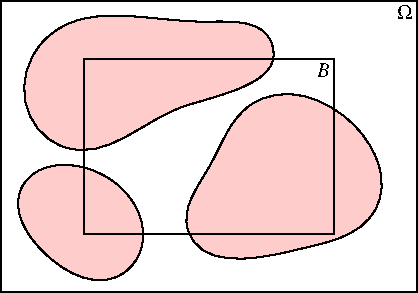
\includegraphics[width=0.8\hsize]{images/algebra-1}
\end{center}
\caption{Ereignisalgebra mit ausgezeichneten Ereignis $B$\label{bedingt1}}
\end{figure}
\begin{figure}
\begin{center}
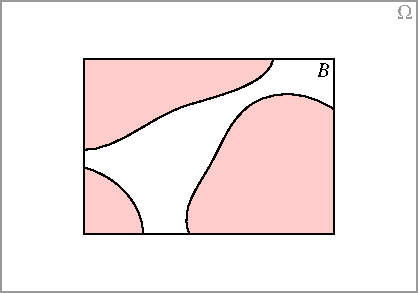
\includegraphics[width=0.8\hsize]{images/algebra-2}
\end{center}
\caption{Ereignisalgebra wie in Abbildung \ref{bedingt1} eingeschr"ankt auf das Ereignis $B$}
\end{figure}
In
\marginpar{\tiny\raggedright Wahrscheilichkeit ``unter Umst"anden''}
der Praxis fragt man oft nach der Verkettung von Umst"anden: hat ein
Patient bessere Heilungschancen wenn er dieses neue Medikament nimmt?
Man k"onnte das auch so formulieren: ist das Ereignis
``Patient wird gesund, unter der Voraussetzung, dass er das Medikament nimmt''
wahrscheinlicher als das Ereignis ``Patient wird gesund''? Wir m"ussen
also aus der Ereignisalgebra der Patienten eine neue bilden, die nur
aus den Patienten besteht, welche das Medikament genommen haben.

Wenn
\marginpar{\tiny eingeschr"ankte Ereignisalgebra}
$(\Omega, {\cal A})$ eine Ereignisalgebra ist, und 
$B\in{\cal A}$ ein Ereignis, dann kann man eine neue Ereignisalgebra
$(\Omega_{|B}, {\cal A}_{|B})$ wie folgt bilden. Die Menge der
Elementarereignisse ist
\[
\Omega_{|B}=B
\]
und die Menge der Ereignisse
\[
{\cal A}_{|B}=\{A\cap B\;|\; A\in{\cal A}\}.
\]
Es w"are noch nachzupr"ufen, dass diese Menge alle Axiome einer
Ereignisalgebra erf"ullt sind, dies wird weiter unten nachgeholt.
Diese Konstruktion macht $B$ zum sicheren Ereignis, d.h. in der ``Welt''
$(\Omega_{|B},{\cal A}_{|B})$ trifft $B$ immer ein.
In $(\Omega_{|B},{\cal A}_{|B})$ muss man also davon ausgehen, dass $B$
bereits eingetroffen ist.

Wenn
\marginpar{\tiny bedingte Wahrscheinlichkeitsfunktion}
nun auf $(\Omega, {\cal A})$ eine Wahrscheinlichkeitsfunktion $P$
gegeben ist, kann man auch $P_{|B}$ bilden, indem man setzt
\begin{equation*}
P_{|B}(A)=\frac{P(A\cap B)}{P(B)},
\end{equation*}
der Nenner $P(B)$ stellt dabei sicher, dass $P_{|B}(\Omega_{|B})=P_{|B}(B)=1$.


\begin{definition}
\label{def-bedingte-wahrscheinlichkeit}
Die bedingte Wahrscheinlichkeit eines Ereignisses $A$ unter der Bedingung
$B$ ist
\[
P(A|B)=\frac{P(A\cap B)}{P(B)}.
\]
\end{definition}

Auch hier w"are nachzupr"ufen, dass die Rechenregeln f"ur eine
Wahrscheinlichkeitsfunktion erf"ullt sind.
Um also die Wahrscheinlichkeit in dieser Welt zu berechnen,
in der $B$ bereits eingetroffen ist, 
muss man $P(A\cap B)$ berechnen k"onnen.
Dies sollte Motivation genug sein, Rechenregeln f"ur
$P(A\cap B)$ aufzustellen, die uns bisher fehlen.

\subsection{Wahrscheinlichkeit von $A\cap B$}
\begin{figure}
\begin{center}
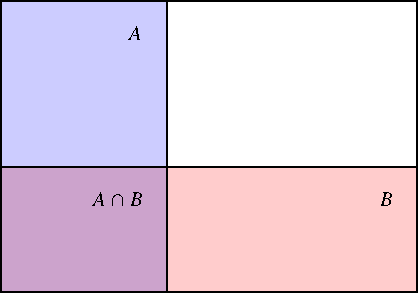
\includegraphics[width=0.8\hsize]{images/abhaengigkeit-1}
\end{center}
\caption{Unabh"angige Ereignisse. Die Ereignisse sind so dargestellt,
dass ihre Wahrscheinlichkeit proportional zur Fl"ache ist. $P(A)$ und $P(B)$
entsprechen dem Teilverh"altnis, in dem $A$ bzw.~$B$ die Seite des grossen
Rechtecks teilen. $P(A\cap B)=P(A)\cdot P(B)$\label{unabhaengig}}
\end{figure}
\begin{figure}
\begin{center}
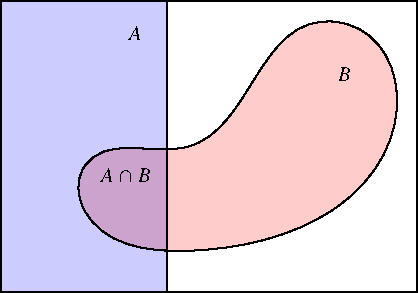
\includegraphics[width=0.8\hsize]{images/abhaengigkeit-2}
\end{center}
\caption{Abh"angige Ereignisse. $P(A\cap B)$ ist offensichtlich viel kleiner
als $P(A)\cdot P(B)$. $A$ wird unwahrscheinlicher, wenn bereits $B$ eingetreten
ist.
\label{abhaengig}}
\end{figure}
Der Grund daf"ur, dass es keine einfache Rechenregel f"ur die Berechung von 
$P(A\cap B)$ aus $P(A)$ und $P(B)$ gibt, wird mit der
Visualisierung der Ereignisse im in einem Venn-Diagramm sofort klar.
Die Elementarereignisse seien so angeordnet, dass $A$ das durch eine
vertikale Strecke abgetrennte linke Teilrechteck von $\Omega$ ist. Ausserdem
sollen Sie so angeordnet sein, dass die Wahrscheinlichkeit dem
Fl"acheninhalt im Diagramm entspricht.

Das Ereignis $B$ ist jetzt im Allgemeinen eine Teilmenge, die sowohl $A$ 
als auch $\bar A$ schneidet. Die Wahrscheinlichkeit $P(A \cap B)$ entspricht
der Fl"ache der Schnittmenge im Diagramm. Im Allgemeinen haben wir
nur aus $P(B)$ nicht gen"ugend Information um zu entscheiden, welche
``Form'' $A\cap B$ hat, wir k"onnen also nicht erwarten, dass wir $P(A\cap B)$
berechnen k"onnen.

Wenn sich $B$ ebenfalls mittels einer horizontalen Strecke als Rechteck
einzeichnen l"asst, dann ist $P(B)$ auch das Teilverh"altnis, in dem
die Strecke die vertikale Kante des Diagrams teilt. Somit kann man $P(A\cap B)$
als Fl"acheninhalt des Schnittrechtecks berechnen: $P(A\cap B)=P(A)\cdot P(B)$.
Die Voraussetzung bedeutet, dass das Eintreffen von $B$ nicht wahrscheinlicher
oder weniger
wahrscheinlich wird, wenn $A$ eintrifft. Das Eintreffen von $B$ h"angt also
nicht mit dem Eintreffen von $A$ zusammen.

\begin{definition}
\label{def-unabhaengige-ereignisse}
Die Ereignisse $A$ und $B$ heissen {\bf unabh"angig}, wenn gilt:
\[
P(A\cap B) = P(A)\cdot P(B).
\]
\end{definition}

Beim W"urfeln sagt die Erfahrung, dass sich ein W"urfel nicht an den
letzten Wurf erinnern kann, d.h. der Ausgang des letzten Wurfes hat
keinen Einfluss auf den n"achsten Wurf. Die Ereignisse ``im ersten
Wurf wird eine 5 gew"urfelt'' und ``im zweiten Wurf wird eine 6 gew"urfelt''
sind also unabh"angig. Die Wahrscheinlichkeit, dass mit einem W"urfel
erst eine 5, dann eine 6 gew"urfelt wird, ist also
\begin{eqnarray*}
P(A\cap B)&=&P(\text{``erster Wurf: 5''}\cap\text{``zweiter Wurf: 6''})\\
&=&P(\text{``erster Wurf: 5''})\cdot P(\text{``zweiter Wurf: 6''})\\
&=&\frac1{36}.
\end{eqnarray*}

\subsection{Bedingte Wahrscheinlichkeit}
Im vorangegangenen Abschnitt wurde bereits die bedingte Wahrscheinlichkeit
$P_{|B}(A)$ konstruiert, die wir auch
\[
P(A|B)=\frac{P(A\cap B)}{P(B)}
\]
schreiben. Die Bedeutung des Symbols $P(A|B)$ ist die folgende. Bei der
Bestimmung der Wahrscheinlichkeit werden nur diejenigen Experimente
ber"ucksichtigt, bei denen das Ereignis $B$ eingetreten ist.
Alle anderen Experimente interessieren nicht.

\subsubsection{Beispiele: Autounf"alle und Alkohol}
Wenn jemand sagt 50\%
der t"odlichen Autounf"alle geschehen unter Alkoholeinfluss, dann
meint er genau genommen eigentlich folgendes. Wir machen ein Experiment,
bei dem wir jeden Autounfall untersuchen. Das Ereignis $T$ umfasst alle
t"odlich ausgehenden Autounf"alle, das Ereignis $A$ all jene, bei denen
Alkohol im Spiel war. Uns interessieren jetzt nur noch die t"odlichen
Unf"alle, also die, bei denen das Ereignis $T$ eingetreten ist. 
Die anderen untersuchen wir gar nicht mehr. Jetzt m"ochten wir die
Wahrscheinlichkeit wissen, dass Alkohol im Spiel war, aber nur noch
bei den t"odlichen Unf"allen. Dies ist $P(A|T)$, also gilt
$P(A|T)=50\% = 0.5$.
$P(T|A)$ ist hingegen ganz etwas anderes. Hier fragt man danach,
wie wahrscheinlich es ist, dass bei einem Autounfall unter Alkoholeinfluss
ein Toter zu beklagen ist.

\subsubsection{Beispiel: Rauchen und Lungenkrebs}
\index{Rauchen}
\index{Lungenkrebs}
In einem Zeitungsartikel gefunden: Die Wahrscheinlichkeit, dass ein Raucher
Lungenkrebs entwickelt, ist 15\%, bei einem Nichtraucher ist sie nur 1\%.
Das Experiment besteht darin, einen Menschen zu beobachten. Einige
davon sind Raucher (Ereignis $R$), einige entwickeln Lungenkrebs (Ereignis $L$).
Betrachtet man nur die Raucher, so ist die Wahrscheinlichkeit f"ur
Lungenkrebs 15\%, also
\[
P(L|R)=0.15
\]
Betrachtet man nur die Nichtraucher, also das Ereignis $\bar R$, findet
man 
\[
P(L|\bar R)=0.01.
\]
Der Artikel liefert aber keine Auskunft dar"uber, wieviele der
Lungenkrebskranken Raucher sind, denn das w"are die Wahrscheinlichkeit
$P(R|L)$.

\subsubsection{Zusammenhang zwischen $P(A\cap B)$, $P(A|B)$ und $P(B|A)$}
In allen drei F"allen geht es um die Wahrscheinlichkeit des Eintretens
von $A$ und von $B$, allerdings jeweils in verschiedenem
Zusammenhang.
\begin{center}
\begin{tabular}{|c|l|c|}
\hline
Wahrscheinlichkeit&"Ubersetzung&Scope\\
\hline
$P(A\cap B)$&\strut Wahrscheinlichkeit, dass $A$ und $B$ eintreten\strut &$\Omega$\\
%\hline
$P(A|B)$&\begin{minipage}[t]{3.0in}\strut Wahrscheinlichkeit, dass $A$ eintritt, wenn $B$ schon eingetreten ist\strut \end{minipage}&$B$\\
%\hline
$P(B|A)$&\begin{minipage}[t]{3.0in}\strut Wahrscheinlichkeit, dass $B$ eintritt, wenn $A$ schon eingetreten ist\strut \end{minipage}&$A$\\
\hline
\end{tabular}
\end{center}
\begin{figure}
\begin{center}
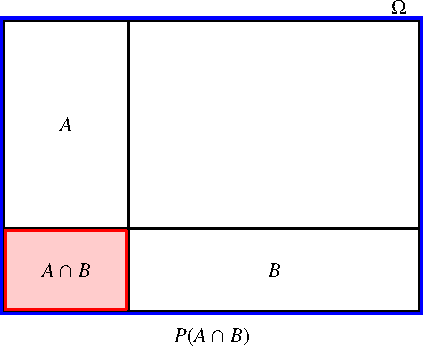
\includegraphics[width=0.3\hsize]{images/abhaengigkeit-3}\quad
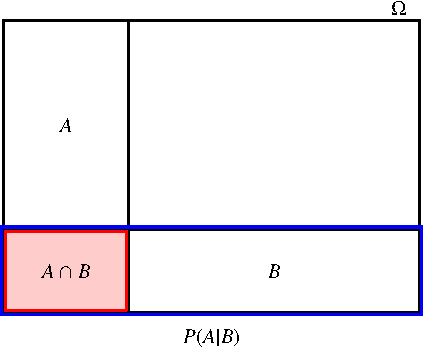
\includegraphics[width=0.3\hsize]{images/abhaengigkeit-5}\quad
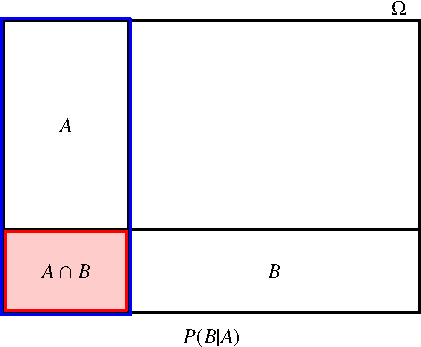
\includegraphics[width=0.3\hsize]{images/abhaengigkeit-4}
\end{center}
\caption{Wahrscheinlichkeit von $A\cap B$ in jeweils anderer Umgebung
\label{condprob}}
\end{figure}

%\subsubsection{Technische Details}
%{\small
%In der Einleitung zu diesem Abschnitt wurde bereits die Konstruktion
%$(\Omega_{|B},{\cal A}_{|B})$ durchgef"uhrt, es ist aber notwendig
%nachzupr"ufen, dass dabei alles mit rechten Dingen zuging, und dass die
%dabei tats"achlich eine Ereignisalgebra konstruiert wurde, und im Falle von
%$P_{|B}$ eine Wahrscheinlichkeitsfunktion.
%
%\begin{satz} Ist $(\Omega,{\cal A})$ eine Ereignisalgebra und
%$B\in{\cal A}$ ein Ereignis, dann ist $(\Omega_{|B},{\cal A}_{|B})$
%eine Ereignisalgebra mit
%\begin{eqnarray*}
%\Omega_{|B}&=&B\\
%{\cal A}_{|B}&=&\{A\cap B\;|\;A\in{\cal A}\}.\\
%\end{eqnarray*}
%\end{satz}
%\begin{proof}[Beweis]
%Es muss nachgepr"uft werden, dass die Vereinigung und die
%Differenz von Ereignissen
%wieder ein Ereignis ist, und dass $\Omega_{|B}\in{\cal A}_{|B}$.
%Dazu bemerken wir zun"achst, dass die Mengen $A\cap B\in {\cal A}_{|B}$
%nat"urlich auch Ereignisse in ${\cal A}$ sind, denn Schnittmengen von
%Ereignissen sind ja wieder Ereignisse.
%
%Eine Folge von Ereignissen $B_i\in{\cal A}_{|B}$ ist also auch eine
%Folge von Ereignissen $B_i\in{\cal A}$, d.h. auch deren Vereinigung
%ist ein Ereignis in ${\cal A}$. Die Vereinigung ist aber auch eine Teilmenge
%von $B$, denn jede einzelne Menge ist darin enthalten. Somit ist
%$$\bigcup_{i=0}^{\infty}B_i=
%B\cap \bigcup_{i=0}^{\infty}B_i\in{\cal A}_{|B}.$$
%Analog folgt, dass mit $C,D\in{\cal A}_{|B}$ auch $C\setminus D$ in ${\cal A}$
%ist, aber auch $C\setminus D\subset B$,
%also $C\setminus D=B\cap(C\setminus D)\in{\cal A}_{|B}$.
%
%Wegen $B=\Omega\cap B\in{\cal A}_{|B}$ sind also alle Axiome erf"ullt.
%\end{proof}
%Zu einer Wahrscheinlichkeitsfunktion $P$ auf $(\Omega,{\cal A})$ haben wir
%bereits die eingeschr"ankte Wahrscheinlichkeitsfunktion $P_{|B}$ konstruiert,
%wir wollen jetzt nachweisen, dass diese die Axiome einer
%Wahrscheinlichkeitsfunktion erf"ullt:
%
%\begin{satz}
%Sei $P$ eine Wahrscheinlichkeitsfunktion auf $(\Omega, {\cal A})$, dann
%ist
%$$P_{|B}(A)=\frac{P(A\cap B)}{P(B)}$$
%eine Wahrscheinlichkeitsfunktion auf $(\Omega_{|B}, {\cal A}_{|B})$.
%\end{satz}
%
%\begin{proof}[Beweis]
%Es sind die drei Axiome f"ur eine Wahrscheinlichkeitsfunktion nachzupr"ufen.
%Sei also $A$ ein Ereignis mit $A\subset B$. Zun"achst zeigen wir, dass 
%$P(A)\le P(B)$. Dazu beachten wir, dass $B=A \cup (B\setminus A)$, wobei
%$A$ und $B\setminus A$ disjunkt sind. Also gilt
%$$P(A)+P(B\setminus A) = P(B).$$
%Da $P(B\setminus A)\ge 0$ folgt daraus $P(A) \le P(B)$.
%Aus dieser Ungleichung folgt jetzt
%$$0\le \frac{P(A)}{P(B)}\le \frac{P(B)}{P(B)}= 1,$$
%d.~h.~das Axiom "uber den Wertebereich ist erf"ullt.
%
%F"ur das sichere Ereignis $B$ in $(\Omega_{|B},{\cal A}_{|B})$ gilt
%$$P_{|B}(B)=\frac{P(B)}{P(B)}=1,$$
%d.~h.~das Axiom betreffend die Wahrscheinlichkeit des sicheren Ereignisses
%ist erf"ullt.
%
%Sei jetzt $A_i$ eine Folge von paarweise disjunkten Ereignissen, die alle
%in $B$ enthalten sind. Dann gilt
%$$P_{|B}\bigl(\bigcup_{i=0}^{\infty}A_i\bigr)
%=P\bigl(\bigcup_{i=0}^{\infty}A_i\bigr)
%=\sum_{i=0}^{\infty}P(A_i)
%=\sum_{i=0}^{\infty}P_{|B}(A_i),$$
%d.~h.~das Axiom betreffend die Vereinigung ist erf"ullt.
%\end{proof}
%
%Somit l"asst sich aus einer Ereignisalgebra und einer
%Wahrscheinlichkeitsfunktion zu einem Ereignis $B$ immer eine
%kleinere Ereignisalgebra bilden, in der das Ereignis $B$ immer
%eintritt. Die zugeh"orige Wahrscheinlichkeitsfunktion $P_{|B}$
%heisst bedingte Wahrscheinlichkeit:
%
%\begin{definition} Ist $(\Omega,{\cal A})$ eine Ereignisalgebra
%und $P$ eine Wahrscheinlichkeitsfunktion, dann heisst die
%Wahrscheinlichkeitsfunktion $P_{|B}$ auf $(\Omega_{|B}, {\cal A}_{|B})$,
%definiert durch
%$$P_{|B}(A)=P(A|B)=\frac{P(A\cap B)}{P(B)}$$
%die bedingte Wahrscheinlichkeit von $A$ unter der Voraussetzung, dass
%$B$ bereits eingetroffen ist.
%\end{definition}
%
%Sind $A$ und $B$ unabh"angige Ereignisse, dann gilt 
%$$P(A|B)=\frac{P(A\cap B)}{P(B)}=\frac{P(A)\cdot P(B)}{P(B)}=P(A),$$
%d.~h.~die Wahrscheinlichkeit, dass $A$ eintritt, ist genau gleich gross
%wie die Wahrscheinlichkeit, dass $A$ unter der Voraussetzung eintritt,
%dass $B$ bereits eingetreten ist. Ob $B$ eingetreten ist oder nicht,
%hat somit auf ein unabh"angiges Ereignis keinen Einfluss.
%
%Die
%\marginpar{\tiny experimentelle Bestimmung bedinger Wahrscheinlichkeiten}
%bedingten Wahrscheinlichkeiten sind das A und O von Meinungsumfragen.
%Bei einer Meinungsumfrage werden ausser der Frage nach der Meinung auch
%Fragen "uber die Person gestellt. Es wird also nicht nur die Wahrscheinlichkeit
%des Ereignises ``Person stimmt zu'' oder ``Person lehnt ab'' gesucht, sondern
%es ist auch die Wahrscheinlichkeit von ``Person ist zwischen 20 und 30 Jahre
%alt'', oder ``Person ist verheiratet'', oder ``Person ist fussballinteressiert''
%bekannt. Aber auch die bedingten Wahrscheinlichkeiten sind bekannt. Wenn
%man nur die Antworten der 20 bis 30 j"ahrigen anschaut, und die relative
%H"aufigkeit der ``Ja''-Antworten in dieser Gruppe bestimmt, hat man
%die bedingte Wahrscheinlichkeit f"ur ``Ja'' ermittelt unter der
%Vorbedingung, dass ``Person ist zwischen 20 und 30 Jahre alt'' bereits
%eingetreten ist.
%}

\subsection{Zerlegung eines Wahrscheinlichkeitsraumes}
Der
\marginpar{\tiny Durchf"uhrung eines Experimentes unter verschiedenen
Rahmenbedingungen}
Begriff der bedingten Wahrscheinlichkeit erm"oglicht,
ein Wahrscheinlichkeitsproblem in m"oglicherweise einfachere, jedenfalls
kleinere Probleme zu zerlegen. Wenn bei einem Experiment zwei Zust"ande
eintreten, die sich gegenseitig ausschliessen, k"onnen wir die 
Wahrscheinlichkeit bestimmen, unter denen die weiteren Resultate
des Experiments eintreten, jedoch unter der Vorbedingung, dass einer
der benannten Zust"ande bereits eingetreten ist. Wenn wir nun auch
noch die Wahrscheinlichkeit jedes Zustandes kennen, m"usste es doch
m"oglich sein, auch die Wahrscheinlichkeit der weiteren Resultate zu
ermitteln.

Im obigen Beispiel der Meinungsumfrage ist anschaulich klar, dass man die
Wahrscheinlichkeit f"ur ``Ja'' berechnen kann, wenn man einerseits die
Wahrscheinlichkeit f"ur ``Ja'' in  jeder Altersklasse kennt, und anderseits
weiss, wie die Altersklassen in der Bev"olkerung verteilt sind.

\begin{figure}
\begin{center}
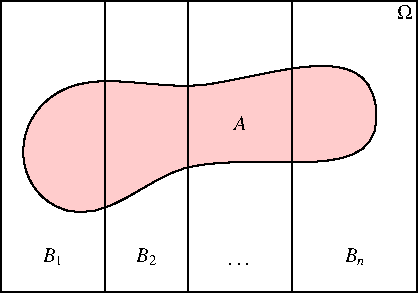
\includegraphics[width=0.8\hsize]{images/total-1.pdf}
\end{center}
\caption{Wahrscheinlichkeitsraum $\Omega$, der sich in die in die
Ereignisse $B_1,B_2,\dots,B_n$ zerlegen l"asst.\label{zerlegung}}
\end{figure}
Wir versuchen das etwas formaler (siehe Abbildung \ref{zerlegung}): Sind $B_i$ mit $1\le i$ paarweise
disjunkte Ereignisse
in einer Ereignisalgebra $(\Omega,{\cal A})$, f"ur welche ausserdem
gilt
\[
\bigcup_{i=0}^{n}B_i = \Omega,
\]
dann kann man die Wahrscheinlichkeit von $A$ aus den bedingten
Wahrscheinlichkeiten der Teile $A\cap B_i$ und $B_i$ wieder zusammensetzen.
Bekannt sind die Wahrscheinlichkeiten
$P(B_i)$, die Wahrscheinlichkeit der Zust"ande, und
$P(A|B_i)$, die Wahrscheinlichkeit, dass $A$ eintritt, unter der Bedingung
das $B_i$ bereits eingetreten ist.
Nach Definition ist $P(A|B_i)=P(A\cap B_i)/P(B_i)$, also
$P(A|B_i)\cdot P(B_i) = P(A\cap B_i)$. Die Vereinigung der Ereignisse
$A\cap B_i$ ist
\[
\bigcup_{i=0}^{n} A\cap B_i=A\cap\bigcup_{i=0}^{n}B_i=A,
\]
und die Mengen $A\cap B_i$ sind disjunkt. Also kann man die Summe ihrer
Wahrscheinlichkeiten mit der Additionsformel ausrechnen:
\[
\sum_{i=0}^{n}P(A\cap B_i)=P\biggl(\bigcup_{i=0}^{n}A\cap B_i\biggr)=P(A).
\]
Andererseits
\marginpar{\tiny Berechnung der Wahrscheinlichkeit aus den bedingten
Wahrscheinlichkeiten}
haben wir oben bereits $P(A\cap B_i)$ bestimmt, wir k"onnen
also einsetzen und erhalten:
\[
P(A)=\sum_{i=0}^{n}P(A|B_i)\cdot P(B_i).
\]
Somit l"asst sich tats"achlich die Wahrscheinlichkeit eines Ereignisses
aus den bedingten Wahrscheinlichkeiten und den Wahrscheinlichkeiten
der Bedingungen errechnen. Wir fassen diese Erkenntnis in folgendem 
Satz zusammen.
\index{Wahrscheinlichkeit!totale}
\begin{satz}
Ist $B_i$ eine Folge paarweise disjunkter Mengen mit $\bigcup_{i=0}^{n}B_i=\Omega$, dann gilt f"ur jedes Ereignis $A$
\[
P(A)=\sum_{i=0}^{n}P(A|B_i)\cdot P(B_i).
\]
\end{satz}
Dieser Satz heisst auch der ``Satz von der totalen Wahrscheinlichkeit'',
da er die Wahrscheinlichkeit eines Ereignisses aus den bedingten
Wahrscheinlichkeiten unter verschiedenen Voraussetzungen und der
Wahrscheinlichkeit des Eintretens dieser Voraussetzungen rekonstruiert.
Dieser Satz ist die ``wahrscheinlichkeitstheoretisch Form einer
Fallunterscheidung'': man kennnt die F"alle $B_i$, und deren Wahrscheinlichkeit
$P(B_i)$, sowie die Wahrscheinlichkeit $P(A|B_i)$, dass $A$ im Falle 
$B_i$ eintritt. Die Formel "uber die Total Wahrscheinlichkeit
liefert daraus wieder $P(A)$.

Wir bemerken noch, dass es gar nicht unbedingt n"otig ist, dass die Mengen
$B_i$ ganz $\Omega$ aussch"opfen, es w"urde auch
gen"ugen, wenn die Wahrscheinlichkeit $0$ ist, dass $A$ eintritt
unter der Bedingung,
dass bereits $\bigcup_{i=0}^{n}B_i$ eingetreten ist.
F"ur den
Experimentator bedeutet das, dass er nur jene Vorbedingungen $B_i$
ber"ucksichtigen muss, unter denen sein Experiment ``funktioniert'',
alle anderen m"oglichen Zust"ande haben keinen Einfluss auf
die Wahrscheinlichkeit seiner Resultate. Man darf beim Experimentieren
also durchaus einzelne Resultate verwerfen, wenn man weiss, was man tut!

\subsubsection{Studienerfolg}
Die folgenden Zahlen sind erfunden, und dienen nur der Illustration
des Prinzips. Eine Statistik hat die Wahrscheinlichkeit f"ur den
Studienerfolg untersucht, und folgende Resultate erhalten.
Die Studierenden setzen sich zusammen aus 60\% BMS, 30\% Kantonssch"uler
und "Ubertritte von anderen Hochschulen. Die Wahrscheinlichkeit
das Studium erfolgreich abzuschliessen, ist f"ur BMS 80\%,
f"ur Kantonssch"uler 90\%, 85\% f"ur die "Ubertreter von anderen
Hochschule. Wie gross ist die Wahrscheinlichkeit f"ur den Studienerfolg?

$\Omega$ ist die Menge aller Studienversuche. 60\% davon bilden das
Ereigns $B$ bestehend aus Studienversuchen, die im Anschluss an die BMS
erfolgen. 30\% machen das Ereignis $K$ mit den Kanti-Abg"angern aus,
10\% das Ereignis $A$ mit "Ubertritten von anderen Hochschulen. Es ist
klar, dass 
\[
\Omega = B \cup K\cup A.
\]
Gefragt ist die Wahrscheinlichkeit des Ereignisses $E$, welches
die erfolgreich abgeschlossenen Studienversuche beinhaltet.
F"ur die Wahrscheinlichkeit gilt nach dem Satz "uber die totale
Wahrscheinlichkeit
\begin{align*}
P(E)&=P(E|B)P(B)+P(E|K)P(K)+P(E|A)P(A).
\\
    &= 80\%\cdot 60\%
     + 90\%\cdot 30\%
     + 85\%\cdot 10\%
\\
&=0.8\cdot 0.6 + 0.9 \cdot 0.3 + 0.85 \cdot 0.1 = 0.835
\end{align*}

\subsubsection{W"urfelspiel}
Wir betrachten nochmals das Beispiel W"urfeln mit zwei W"urfeln, wobei
bei einem Pasch im ersten Wurf noch genau einmal gew"urfelt wird. 
Wir m"ochten die Wahrscheinlichkeit berechnen, dass die totale Augensumme
mindestens 10 ist. Wir nennen dieses Ereignis $Z$.

Zun"achst kann man unterteilen in den Fall, dass im ersten Wurf
ein Pasch geworfen wird. Es gilt nach dem Satz "uber die totale
Wahrscheinlichkeit
\[
P(Z) = P(Z|P) P(P) + P(Z|\bar P) P(\bar P).
\]
Selbstverst"andlich ist $P(\bar P)=1-P(P)$, so dass man $P(Z)$ bereits
vereinfachen kann:
\[
P(Z) = P(Z|P) P(P) + P(Z|\bar P) (1-P(P)).
\]
Man kann aber das Ereignis $P$ noch weiter unterteilen in die
Ereignisse $P_k$, mit $1\le k\le 6$, also
\begin{align*}
P(P)&=
P(P_1)+
P(P_2)+
P(P_3)+
P(P_4)+
P(P_5)+
P(P_6)
\\
P(Z|P)
&=
P(Z|P_1)P(P_1|P)+
P(Z|P_2)P(P_2|P)+
P(Z|P_3)P(P_3|P)
\\
&\qquad +
P(Z|P_4)P(P_4|P)+
P(Z|P_5)P(P_5|P)+
P(Z|P_6)P(P_6|P)
\end{align*}
Die Ereignisse haben wir auch fr"uher schon untersucht, daraus kann
man einige Wahrscheinlichkeiten bereits ablesen:
\begin{align*}
P(Z|P_6)&=1\\
P(Z|P_5)&=1\\
P(Z|P_4)&=1
\end{align*}
denn in allen diesen F"allen erreicht man mit dem zweiten Wurf mit
Sicherheit zehn oder mehr.

\subsection{Wahrscheinlichkeitsvektoren und -matrizen}
Der Satz von der totalen Wahrscheinlichkeit kann auch in Matrixform
geschrieben werden:
\begin{align*}
P(A)&=P(A|B_1)P(B_1)+\dots+P(A|B_n)P(B_n)
=
\begin{pmatrix}
P(A|B_1)&\dots&P(A|B_2)
\end{pmatrix}
\begin{pmatrix}
P(B_1)\\\vdots\\P(B_n)
\end{pmatrix}
\end{align*}
Der Spaltenvektor
\[
\begin{pmatrix}
P(B_1)\\\vdots\\P(B_n)
\end{pmatrix}
\]
hat die Eigenschaften, dass alle seine Eintr"age zwischen $0$ und $1$
liegen, und ihre Summe $1$ gibt.
\index{Wahrscheinlichkeitsvektor}
Ein solcher Vektor heisst {\it Wahrscheinlichkeitsvektor}.

Die Matrizenschreibweise erlaubt, auch die totalen Wahrscheinlichkeiten
f"ur mehrere Ereignisse $A_1,\dots,A_m$ gleichzeitig zu berechnen:
\[
\begin{pmatrix}
P(A_1)\\
P(A_2)\\
\vdots\\
P(A_m)
\end{pmatrix}
=
\begin{pmatrix}
P(A_1|B_1) & P(A_1|B_2) & \dots &P(A_1|B_n)\\
P(A_2|B_1) & P(A_2|B_2) & \dots &P(A_2|B_n)\\
\vdots     & \vdots     & \ddots&\vdots\\
P(A_m|B_1) & P(A_m|B_2) & \dots &P(A_m|B_n)\\
\end{pmatrix}
\begin{pmatrix}
P(B_1)\\
P(B_2)\\
\vdots\\
P(B_n)
\end{pmatrix}
\]
Sind die Ereignisse $A_i$ ebenfalls paarweise disjunkt und decken ganz
$\Omega$ ab, dann sind auch die Spalten von der Matrix $(P(A_i|B_j))$
jeweils Wahrscheinlichkeitsvektoren. 
\index{Wahrscheinlichkeitsmatrix}
Eine solche Matrix heisst {\it Wahrscheinlichkeitsmatrix}.

\subsection{Satz von Bayes} \label{satz-von-bayes}
\index{Bayes, Satz von}
F"ur zwei beliebige Ereignisse mit $A$ und $B$ mit nicht verschwindender
Wahrscheinlichkeit gilt
\[
P(A|B)\cdot P(B)= P(A\cap B)=P(B|A)\cdot P(A),
\]
und es folgt
\[
P(A|B)=\frac{P(B|A)\cdot P(A)}{P(B)}.
\]
Dieser Zusammenhang ist bekannt als der Satz von Bayes:
\begin{satz}[Satz von Bayes]
F"ur zwei Ereignisse $A$ und $B$ mit $P(B)\ne0$ gilt
\[
P(A|B)=\frac{P(B|A)\cdot P(A)}{P(B)}.
\]
\end{satz}
Die Bedeutung dieses Satzes besteht darin, dass er die Schlussrichtung
umzukehren erlaubt. Die bedingte Wahrscheinlichkeit $P(A|B)$ ist ja die
Wahrscheinlichkeit, dass ein das Ereignis $A$ eintritt, wenn $B$ bereits
eingetreten ist. Sie erlaubt, eine Wette einzugehen, dass $A$ eintreten
wird, wenn $B$ bereits eingetreten ist. Der Satz von Bayes erm"oglicht
also, auch eine Wette f"ur $B$ einzugehen, wenn $A$ bereits eingetreten
ist.
Im Gegensatz zur Schlussweise in der Logik, die niemals umkehrbar ist,
kann man auf Wahrscheinlichkeiten basierende Schl"usse umkehren.

\subsubsection{Was bedeutet ein positiver HIV-Test?}
\begin{figure}
\begin{center}
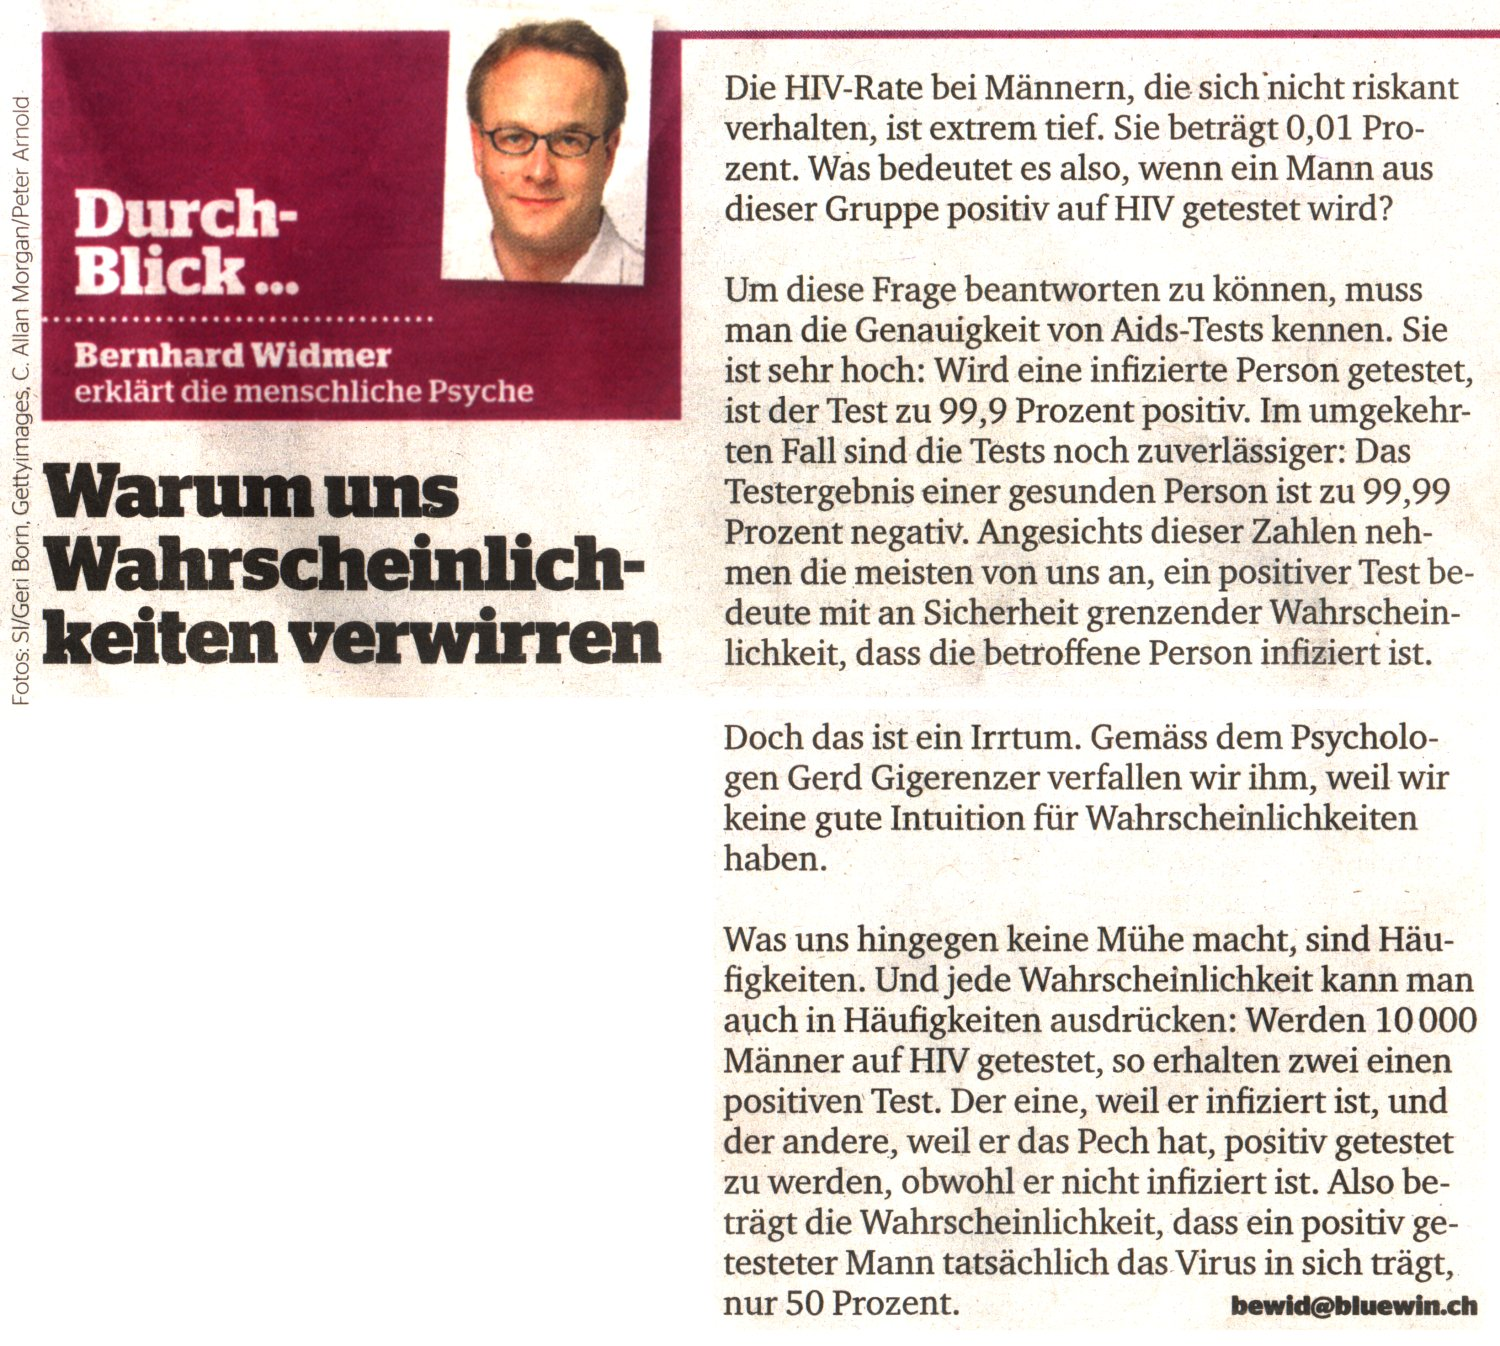
\includegraphics[width=\hsize]{graphics/aids-300}
\end{center}
\caption{``Blick am Abend'' vom 12.~August 2008\label{aids}}
\end{figure}
Im ``Blick am Abend'' vom 12.~August 2008 erschien der Artikel in Abbildung 
\ref{aids} mit dem Titel ``Warum uns Wahrscheinlichkeiten verwirren''.
Darin ist von folgenden Ereignissen die Rede, die sich auf sich nicht riskant
verhaltende M"anner ($=\Omega$) beziehen.
\index{HIV-Test}
\begin{enumerate}
\item Ereignis $H$: Ein Mann ist HIV-infiziert.
\item Ereignis $T$: ein HIV-Test ergibt ein positives Resultat.
\end{enumerate}
Der Artikel teilt uns zudem ein paar Wahrscheinlichkeiten mit:
\begin{itemize}
\item HIV-Rate bei M"annern, die sich nicht riskant verhalten:
$P(H)=0.0001$.
\item Wahrscheinlichkeit, dass bei einer infizierten Person der Test
ein positives Resultat ergibt: $P(T|H)=0.999$.
\item Wahrscheinlichkeit, dass bei einer gesunden Person der Test negativ
ist: $P(\bar T|\bar H)=0.9999$.
\end{itemize}
Wie gross ist die Wahrscheinlichkeit, dass ein sich nicht riskant verhaltender
Mann tats"achlich HIV hat, wenn er einen positiven HIV-Test hat? Wie
gross ist $P(H|T)$?

Der Satz von Bayes liefert die Antwort:
\begin{equation}
P(H|T)=\frac{P(T|H)\cdot P(H)}{P(T)}
\label{aidsprobability}
\end{equation}
Darin sind fast alle Gr"ossen direkt aus dem Artikel ablesbar, nur $P(T)$ muss
noch bestimmt werden. Dazu dient der Satz "uber die totale Wahrscheinlichkeit,
den wir auf die Tatsache anwenden, dass ein sich nicht riskant verhaltender
Mann entweder HIV hat oder nicht: $\Omega=H\cup \bar H$.
\begin{align*}
P(T)
&=P(T|H)\cdot P(H)+P(T|\bar H)\cdot P(\bar H)\\
&=P(T|H)\cdot P(H)+(1-P(\bar T|\bar H))\cdot (1 - P(H))\\
&=0.999\cdot 0.0001+(1-0.9999)\cdot(1-0.0001)\\
&=0.00019989\simeq 0.0002
\end{align*}
Eingesetzt in (\ref{aidsprobability}) ergibt sich jetzt das Resultat
\[
P(H|T)=\frac{0.999\cdot 0.0001}{0.0002}=.4995\simeq 0.5
\]
oder mit anderen Worten, auch wenn der HIV-Test positiv ist, ist
die Wahrscheinlichkeit f"ur einen sich nicht riskant verhaltenden Mann,
tats"achlich HIV-infiziert zu sein, nur $50\%$.

\subsubsection{Weitere Beispiele}
Im Anhang \ref{spamfilter} wird als weiteres Anwendungsbeispiel ein Spamfilter
beschrieben. Der Google Pagerank, beschrieben in Anhang \ref{pagerank},
ist eine Anwendung der bedingten Wahrscheinlichkeit und des Satzes von
der totalen Wahrscheinlichkeit auf Suchmaschinen.

%\subsection{Der Viterbi-Algorithmus}
%Wir stellen uns einen "Ubertragungskanal vor, der endlich viele
%verschiedene Symbole "ubertragen kann.
%In diskreten, mit nat"urlichen Zahlen numerierten Zeitschritten,
%werden Symbole $A_i$ "ubermittelt.
%Infolge Rauschens k"onnen
%die Symbole nicht immer zuverl"assig erkannt werden, sondern
%nur mit einer gewissen Wahrscheinlichkeit.  Es wird also im $k$-ten
%Schritt das Symbol $a_k$ erkannt. $P(a|A)$ ist die Wahrscheinlichkeit,
%dass $a$ erkannt wird wenn tats"achlich $A$ "ubermittelt wurde.
%
%Die "ubermittelten Zeichen sind nicht zuf"allig, vielmehr sind
%gewisse Abfolgen von Zeichen wahrscheinlicher als andere. Die
%Wahrscheinlichkeit, $P(A_k|A_{k-1})$ h"angt nur von den beiden
%Zeichen ab, die "ubermittelt wurden. 
%
%{\bf 1. Schritt:} Ein Zeichen ist "ubermittelt worden, und das Zeichen
%$a_1$ ist erkannt worden. Welches Zeichen wurde gesendet?
%
%Die Wahrscheinlichkeit, dass das Zeichen $a$ erkannt wird, wenn
%$A$ "ubermittelt wird, $P(a|A)$. Wir m"ochten aber
%die Wahrscheinlichkeit, dass $A$ gesendet wird, wenn $a$ erkannt worde
%ist, also $P(A|a)$. Nach dem Satz von Bayes
%ist
%$$P(A|a)=\frac{P(a|A)\cdot P(A)}{P(a)}$$
%Wenn wir annehmen, dass die "ubermittelten Zeichen genau gleich
%wahrscheinlich sind wie die erkannten Zeichen, der Erkennungsmechanismus
%also keine Zeichen bevorzugt, dann k"urzen sich die einfachen
%Wahrscheinlichkeiten weg, und wir bekommen 
%$$P(A|a)=P(a|A).$$
%Daraus k"onnen wir schliessen, dass das wahrscheinlichste "ubermittelte
%Zeichen $A$ jenes ist, f"ur welches $P(a|A)$ maximal wird.
%
%{\bf 2. Schritt: } Wir nehmen jetzt an, dass bereits $k-1$ Beobachtungen
%aufgezeichnet worden sind, und dass bereits berechnet wurde, mit
%welcher Wahrscheinlichkeit $P(A_{k-1})$
%die unter diesen Beobachtungen wahrscheinlichste
%Abfolge von gesendeten Zeichen mit $A_{k-1}$ endet.
%
%\begin{enumerate}
%\item Wahrscheinlichkeit, dass der wahrscheinlichste Pfad zu einem
%in $X$ enden Pfad fortgesetzt wird:
%$$P(X|A_{k-1}) P(A_{k-1}).$$
%\item Wahrscheinlichkeit, dass der nach $X$ fortgesetzte Pfad 
%als $a_k$ erkannt wird
%\begin{equation}
%P(a_k|X) P(X|A_{k-1}) P(A_{k-1})
%\label{viterbi}
%\end{equation}
%\item
%Die wahrscheinlichste Fortsetzung des Pfades unter Ber"ucksichtigung
%der neuen Beobachtung $a_k$ ist also jenes $X$, welches
%(\ref{viterbi})
%maximiert.
%\end{enumerate}
%
%Wir beschreiben, wie sich der Algorithmus f"ur 
%Symbole $A\in\{1,\dots,n\}$
%durch\-f"uhren l"asst.
%\begin{enumerate}
%\item Array {\tt p[n]} allozieren, er enth"alt die aktuellen Werte
%von $P(A_k)$.
%\item Beobachtung $a_1$ verwerten: setze 
%$$\text{\tt p[I]}= P(a_1|{\tt I})$$
%\item Der wahrscheinlichste Zustand unter den bisher erfolgten Beobachtungen
%ist dasjenige {\tt J}, welches {\tt p[J]} maximiert.
%\item \label{viterbiloop}Neue Beobachtung $a_k$: Berechne die Werte
%\begin{equation}
%P(a_k|{\tt I})
%\cdot
%P({\tt I}|{\tt J})
%\cdot
%\text{\tt p[J]}
%\label{viterbimax}
%\end{equation}
%\item Finde {\tt I} derart, dass (\ref{viterbimax}) maximal wird, setze
%${\tt J}={\tt I}$.
%\item Gehe zu Schritt \ref{viterbiloop}.
%\end{enumerate}
%Dieser Algorithmus findet also diejene Folge von Zeichen, die am besten
%zu den erkannten Zeichen ``passt''. Nicht immer findet er die
%richtige Folge von Zeichen, aber es ist sehr wahrscheinlich, dass er
%viele Zeichen hintereinander richtig erkennt, und damit verst"andliche
%S"atze oder Datenbl"ocke rekonstruieren kann.
%
%
%\section{Ein paar technische Details}
%Solange man mit endlichen oder diskreten Mengen arbeitet, ist jede beliebige
%Teilmenge ein mathematisch sinnvolles Ereignis.
%In einigen der oben diskutierten F"allen ist die Menge $\Omega$ aber sehr
%gross, meistens "uberabz"ahlbar. In diesen F"allen ist es etwas viel
%verlangt, wenn die Funktion $P$ f"ur jede beliebige Teilmenge  von $\Omega$
%definiert sein soll, und ausserdem noch alle Axiome erf"ullt sein sollen.
%In der Tat wurden pathologische Mengen gefunden, f"ur die die Additionsregel
%f"ur jede sinnvolle Definition von $P$ nicht erf"ullbar ist.
%
%Aus technischen mathematischen Gr"unden muss daher die Menge der Ereignisse
%eingeschr"ankt werden. Dabei m"ussen die Rechenregeln f"ur $P$ erhalten
%bleiben. Dazu muss die leere Menge, die ganze Menge, die Komplementmenge
%einer Menge und jede endliche Vereinigung und jeder endliche Durchschnitt
%von Ereignissen wieder ein Ereignis sein.
%
%Auch in der Analysis gibt man den Zahlenmengen eine zus"atzliche
%Struktur, um den Begriff des Grenzwertes exakt formulieren zu k"onnen.
%Man arbeitet dabei meist mit offenen Intervallen, also mit Mengen der Form
%$$U_\varepsilon(x) = \{ y\in\mathbb R\;|\; |x-y|<\varepsilon\}.$$
%Eine Folge $(a_n)_{n\in\mathbb N}$ konvergiert zum Beispiel gegen den Grenzwert
%$a$ wenn zu jedem $\varepsilon > 0$ ein $N$ existiert so dass
%$a_k\in U_\varepsilon(a)$ wenn nur $a > N$ ist. Oder eine Funktion $f$ ist
%im Punkt $x$ stetig,
%wenn f\"ur jedes $\varepsilon > 0$ ein $\delta > 0$ existert,
%so dass $f$ die Punkte, die gen"ugend nahe bei $x$ sind, auch  nahe an $f(x)$
%abbildet:
%$$f(U_\delta(x)) \subset U_\varepsilon(f(x)).$$
%Den $U_\varepsilon(x)$ ist gemeinsam, dass sie alle offene B"alle sind,
%d.h.~mit jedem Punkt ist auch ein kleiner Ball um den Punkt in der Menge
%enthalten. Es gibt nat"urlich noch viele weitere offene Mengen, durch
%Vereinigung und endliche Durchschnitte k"onnen aus bekannten offenen Menge
%weitere offene Mengen erzeugt werden.
%
%Man kann die Begriffe Grenzwert und Stetigkeit vollst"andig aufbauen, wenn
%man weiss, was ``nahe'' heissen soll. Man k"onnte dazu einen Abstandsbegriff
%definieren, und Mengen $U_\varepsilon(x)$ f"ur beliebige Mengen betrachten,
%in denen so ein Abstandsbegriff definiert ist. Es geht aber auch allgemeiner.
%Statt sich damit abzum"uhen, den Abstandsbegriff zu kl"aren, kann man auch
%einfach die Menge aller offenen Mengen festlegen. Konvergenz w"urde dann zum
%Beispiel so definiert: die Folge $(a_k)_{k\in\mathbb N}$ ist konvergent, wenn
%es zu jeder offenen, $a$ enthaltenden Menge $U\ni a$ ein $N(U)$ gibt
%sodass $a_k\in U$ sobald $k>N(U)$. Stetigkeit ist noch einfacher: die Funktion
%$f$ ist stetig, wenn f"ur jede offene Menge $U$ im Wertebereich die
%Urbildmenge $f^{-1}(U)$ im Definitionsbereich offen ist.
%
%W"ahrend ein Abstandsbegriff in den meisten Anwendungen durchaus kein
%un"uberwindliches Hindernis ist, f"allt uns in der Wahrscheinlichkeitsrechnung
%bereits die Beschreibung aller Elementarereignisse schwer. Darauf nun
%auch noch f"ur alle von der Anwendung suggerierten $P$ eine Menge von
%Teilmengen $\Omega$ zu finden, welche die Ereignisse beschreiben k"onnte,
%wird kaum einfacher sein. Daher gehen wir den umgekehrten Weg, und geben
%die Menge $\Omega$ vor, verlangen aber zus"atzliche Eigenschaften, die
%uns garantieren, dass wir mit den $P$ nach Regeln rechnen k"onnen, die uns
%plausibel und nat"urlich erscheinen.
%
